\documentclass[whitelogo,12pt]{tudelft-report}
\usepackage{natbib}
\usepackage{changes}

\usepackage{color}
\definecolor{covercolor}{RGB}{235,250,254}
\usepackage{graphicx}
\graphicspath {{figures/}}

\begin{document}
\captionsetup{justification=centering}
%% Use Roman numerals for the page numbers of the title pages and table of
%% contents.
\frontmatter

%% Uncomment following 19 lines for a cover with a picture on the lower half only
 \title[black]{MICA}
 \subtitle[tudelft-cyan]{Music Identifying and Classifying Application}
 \author[tudelft-white]{Jiaxi Li\\Weichen Zhang\\Yuan Fang}
 %\affiliation{Technische Universiteit Delft}
% \coverimage{cover.jpg}
 \titleoffsetx{10cm}
 \titleoffsety{10cm}
 \afiloffsetx{1cm}
 \afiloffsety{18cm}
 %\covertext[tudelft-white]{
%    \textbf{Cover Text} \\
%    possibly \\
%    spanning 
%    multiple 
%    lines
%    \vfill
%    ISBN 000-00-0000-000-0
% }
 \setpagecolor{covercolor}
 %\makecover
\let\cleardoublepage\clearpage

%% Uncomment following 16 lines for a cover with a picture on the lower half only
%\title[tudelft-white]{Title}
%\subtitle[tudelft-black]{Optional subtitle}
%\author[tudelft-white]{J.\ Random Author}
%\affiliation{Technische Universiteit Delft}
%\coverimage{tank.jpg}
%\covertext[tudelft-white]{
%    \textbf{Cover Text} \\
%    possibly \\
%    spanning 
%    multiple 
%    lines
%    \vfill
%    ISBN 000-00-0000-000-0
%}
%\setpagecolor{tudelft-cyan}
%\makecover[split]


%% Include an optional title page.

%------------------------------------------------------------------------------------------------------------------------------------
%
%							TITLE PAGE
%
%------------------------------------------------------------------------------------------------------------------------------------
\begin{titlepage}
\begin{center}

%% Insert the TU Delft logo at the bottom of the page.

%% Print the title in cyan.
{\makeatletter
\largetitlestyle\fontsize{64}{94}\selectfont\@title
%\largetitlestyle\color{tudelft-cyan}\Huge\@title
\makeatother}

%% Print the optional subtitle in black.
{\makeatletter
\ifx\@subtitle\undefined\else
    \bigskip
   {\tudsffamily\fontsize{22}{32}\selectfont\@subtitle}    
    %\titlefont\titleshape\LARGE\@subtitle
\fi
\makeatother}

\bigskip
\bigskip
\bigskip
\bigskip
\bigskip
\bigskip

by
%door

\bigskip
\bigskip
\bigskip


%% Print the name of the author.
{\makeatletter
%\largetitlefont\Large\bfseries\@author
\largetitlestyle\fontsize{26}{26}\selectfont\@author
\makeatother}

\bigskip
\bigskip
\bigskip
\bigskip
\bigskip
\bigskip


\Large COMP5425
%ter verkrijging van de graad van Master of Science

Multimedia Retrieval
%aan de Technische Universiteit Delft,

Project Final Report
%in het openbaar de verdedigen op dinsdag 1 januari om 10:00 uur.

%\vfill
\bigskip
\bigskip
\bigskip
\bigskip
\bigskip
\bigskip
\bigskip
\bigskip

\begin{tabular}{rll}
    Project Duration: & 6 Weeks\\
    Project Start Date: 			& 13/04/2016\\
    Project End Date:   			& 25/05/2016
\end{tabular}
%% Only include the following lines if confidentiality is applicable.

\bigskip
\bigskip
%\emph{This thesis is confidential and cannot be made public until December 31, 2013.}
%\emph{Op dit verslag is geheimhouding van toepassing tot en met 31 december 2013.}

\bigskip
\bigskip
%An electronic version of this thesis is available at \url{http://repository.tudelft.nl/}.
%\\[1cm]

%\centering{\includegraphics{cover/logo_black}}


\end{center}

%\begin{tikzpicture}[remember picture, overlay]
%    \node at (current page.south)[anchor=south,inner sep=0pt]{
%        \includegraphics{cover/logo_black}
%    };
%\end{tikzpicture}

\end{titlepage}
\let\cleardoublepage\clearpage

%\chapter*{Preface}
\setheader{Preface}

Preface\ldots

\begin{flushright}
{\makeatletter\itshape
    \@author \\
    Delft, January 2013
\makeatother}
\end{flushright}



\tableofcontents

%% Use Arabic numerals for the page numbers of the chapters.
\mainmatter

%------------------------------------------------------------------------------------------------------------------------------------
%
%							CONTENT
%
%------------------------------------------------------------------------------------------------------------------------------------

%------------------------------------------------------------------------------------------------------------------------------------
%							INTRODUCTION
%------------------------------------------------------------------------------------------------------------------------------------
\chapter{Introduction}
\section{Motivation}
The rapid growth in technology is greater than ever nowadays. In this context, music is getting more and more popular, and an increasing number of music has been infiltrated into lives of people and influencing them in different forms. With the development of the network and digitization technology, people are surrounded by music at all times. However, people may enjoy particular music without knowing what this song is or what it consists of. Therefore, identifying songs of interests becomes an executable and reasonable motivation for developing applications to suit this objective.

\section{Project} \label{project}
Due the over-variety of music, this project is mainly focusing on Classical Music. There are three major functionality in this deliverable: match incoming music (through files and recordings) with our database, classify instrument played within music (through files and recordings), and rate the music played by yourself.

\subsection{Searching}
Similar to \textit{Shazam}\footnote{\url{http://www.shazam.com}}, we capture a piece of music clip from either microphone or unrecognized music file, and produce the best matching result in our database.

\subsection{Instrument Classification}
Beside the music name, what instrument played within music interests people. This project provides the ability of identifying instruments through either an unclassified file or microphone on you computer.

\subsection{Rate Yourself}
What more than matching and classifying is having the fun by practicing your own skills. Select the favorite  song in the database, and upload personal plays (or through microphone). Then, score will be showing up, and parts that are not played well is pointed out to users on the screen.

%------------------------------------------------------------------------------------------------------------------------------------
%							Project specification
%------------------------------------------------------------------------------------------------------------------------------------
\chapter{Project Specification}
\section{Group Work}
The three major functionality, searching, instrument classifying and rating, are divided and assigned to Weichen Zhang, Jiaxi Li, Yuan Fang respectively. While everyone in the group is working individually with his part, GUI integration is conducted by all of the members regards to corresponding functionality.

\section{Working Environment}
\subsection{Source Code}
Major functionality is implemented in pure $Python$. GUI is built with python interface dependencies $pygame$\footnote{\url{http://www.pygame.org/}} and $Tkinter$\footnote{\url{https://docs.python.org/2/library/tkinter.htm}}.

\section{Related Work}
\label{relatedwork}
Burnett et al. mentioned in \cite{burnett2006}, "an audio fingerprint is a condensed digital summary, deterministically generated from an audio signal, and then can be used to identify audio samples or locate similar items in audio database in a very short time". With this determination of technique, Kim et al. then has proposed an algorithm for extracting music fingerprints directly from the audio signal in \textit{IEEE International Conference} in 2008\cite{kim2008}. Moreover, she had concluded that this proposed algorithm outperformed the conventional state-of-art identification system. After that, there are various methodologies proposed to augment precision and reliability of audio fingerprints.
\\
\indent In 2013, Lee et al. \cite{lee2013} pointed out the inefficiency in Haitsma's fingerprint system\cite{kalker2009}. The audio fingerprinting system provided by Haitsma uses a lookup table to identify the candidate songs in the database, which contains the sub-fingerprints of songs, and searches the candidates to find a song whose bit error rate is the lowest. However, the communication between system and database is extremely frequent which can result in the lost of sub-fingerprint duo to heavily degraded input signal. Lee, on the other had, solves this difficulties by reducing the number of database accesses using an partitioned method on each song.
\\
\indent In the last few years, audio fingerprint has been successfully applied and developed in repeating pattern detection\cite{chen2015}, speech recognition \cite{sharifi2015}, and audio content recognition\cite{jo2016}.
\\
\\
For the purpose of recognizing instrument, Li et al. compared few approaches of extracting instrument within an audio, including convolutional neural networks (CNN) and Mel-frequency cepstral coefficients (MFCCs) \cite{li2015}. 
\\
\indent MFCC computation technique is derived from a type of cepstral representation of the audio clip. It utilizes discrete cosine transform (DCT) for decorrelating log energies of filter bank output \cite{sahidullah2012}. Then resulting log energies and filter banks can be used to calculating a set of coefficients that can best represent an audio. In fact, Bhalke et al. published a paper in \textit{Digital Signal Processing Journal} in 2013 \cite{bhalke2013} and described the combination of higher order moments and MFCC improves recognition accuracy by more than 8\% comparing to convention methodologies.

%------------------------------------------------------------------------------------------------------------------------------------
%							Analysis
%------------------------------------------------------------------------------------------------------------------------------------
\section{Problem Analysis}
\subsection{Feature Extraction}
The first step of audio recognition is to extract features. Mel-Frequency Cepstral Coefficents (MFCCs) is one of the most widely used technique for select features in speeches and speakers. As Ganchev et al. mentioned in \cite{ganchev2005}, different implementations may result in different performance. Therefore, the implementation of MFCCs in this project is carried out on our own in following steps:
\begin{quote}
1. Frame signal into short frames.\\
2. Calculate power spectrum for each frame.\\
3. Generate and apply Mel filter banks and energies to power spectrum.\\
4. Compute logarithm of all filter bank energies.\\
5. Transform resulting log filter bank energies to DCT\footnote{Discrete cosine transform}.\\
6. Keep 13 coefficients, and discard others.
\end{quote}
Note that above steps are high level introduction for implementation, a more detailed description will be given in Section~\ref{IC}.

\subsection{Semi-Real-Time System}
As mentioned in the Section~\ref{project}, the objective of project is to build an application that can retrieve relevant audio in database to match an unknown source and identify instruments played in it. In order to achieve this goal, this application has to perform selected tasks within a reasonable time. Similar to $Shazam$, our application allows user to record a clip of audio and then perform the selected task. Besides, tasks can also be executed on a selected audio file by browsing file system.


%------------------------------------------------------------------------------------------------------------------------------------
%							Implementation
%------------------------------------------------------------------------------------------------------------------------------------
\chapter{Implementation}
\section{Instrument Classification} \label{IC}
\subsection{MFCCs}
As the standards mentioned in \cite{murty2006}, the signal of audio is framed in to 25 $ms$ and number frame step is 10 $ms$ which allows some overlap between frames. That is, for an audio whose sample rate is 16 $kHz$, it has 400 samples after the framing process.

Before power spectrum is computed, Discrete Fourier Transform (DFT) is applied to each frames as follow:
\begin{equation}
S_i(k) = \displaystyle \sum^{N}_{n=1}s_i(n)h(n)e^{\dfrac{-j2\pi kn}{N}} \quad \quad k = 1,2,...,K
\end{equation}
where $s(n)$ is time domain signal and $s_i(n)$ represents segmented frames. $h(n)$ indicates a $N$  sample long analysis window, and $K$ denotes length of DFT. Therefore, power spectrum $P_i(k)$ for each frame is given by:
\begin{equation}
P_i(k) = \dfrac{1}{N}(S_i(k))^2
\end{equation}

Mel filter bank is generated using 26 triangular filters (standard), and then resulting filter bank is applied to each power spectrum we had calculated above and filter bank energies are computed through multiplying each filter bank with power spectrum, then add up the coefficients. Once this is calculated, each filter bank will be left with 26 numbers indicating how much energy is in it. The example results of power spectrum and filter banks are illustrated in Figure~\ref{fig:filter}.
\begin{figure}
\centering
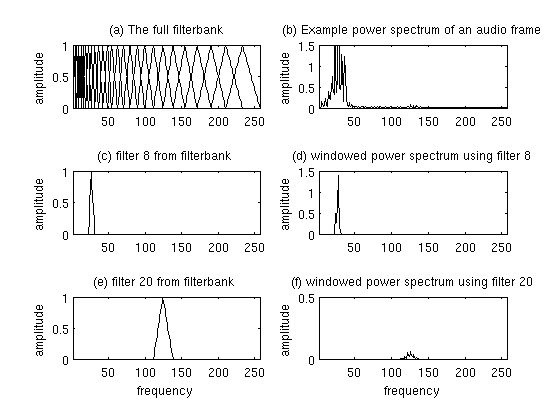
\includegraphics[scale=0.7]{mel_filterbank_example}
%\captionsetup{justification=centering}
\caption{Graphical illustration of power spectrum and filter banks.}
\label{fig:filter}
\end{figure}
The essential steps for calculating filter bank can be found in \cite{milner2002}.

Next step is doing logarithm on 26 filter bank energies. Once log energies are compute, Discrete Cosine Transform (DCT) is applied on resulting 26 energies to generate same number of cepstral coefficients. At last, in this project, only 14 out of 26 lowest coefficients are kept for the purpose of classifying.

As Li pointed out in \cite{li2015}, after MFCCs of each song in database are computed, we train our data with Random Forest which is a widely used classification technique implemented in $sci$-$kit$ $learn$\footnote{\url{http://scikit-learn.org}}. 

\subsection{Storyboard Walk Through}
The walk through for operating instrument classification is shown in Figure~\ref{fig:if} and~\ref{fig:im} from left to right, top to bottom.

\begin{figure}[!htb]
\minipage{0.497\textwidth}
  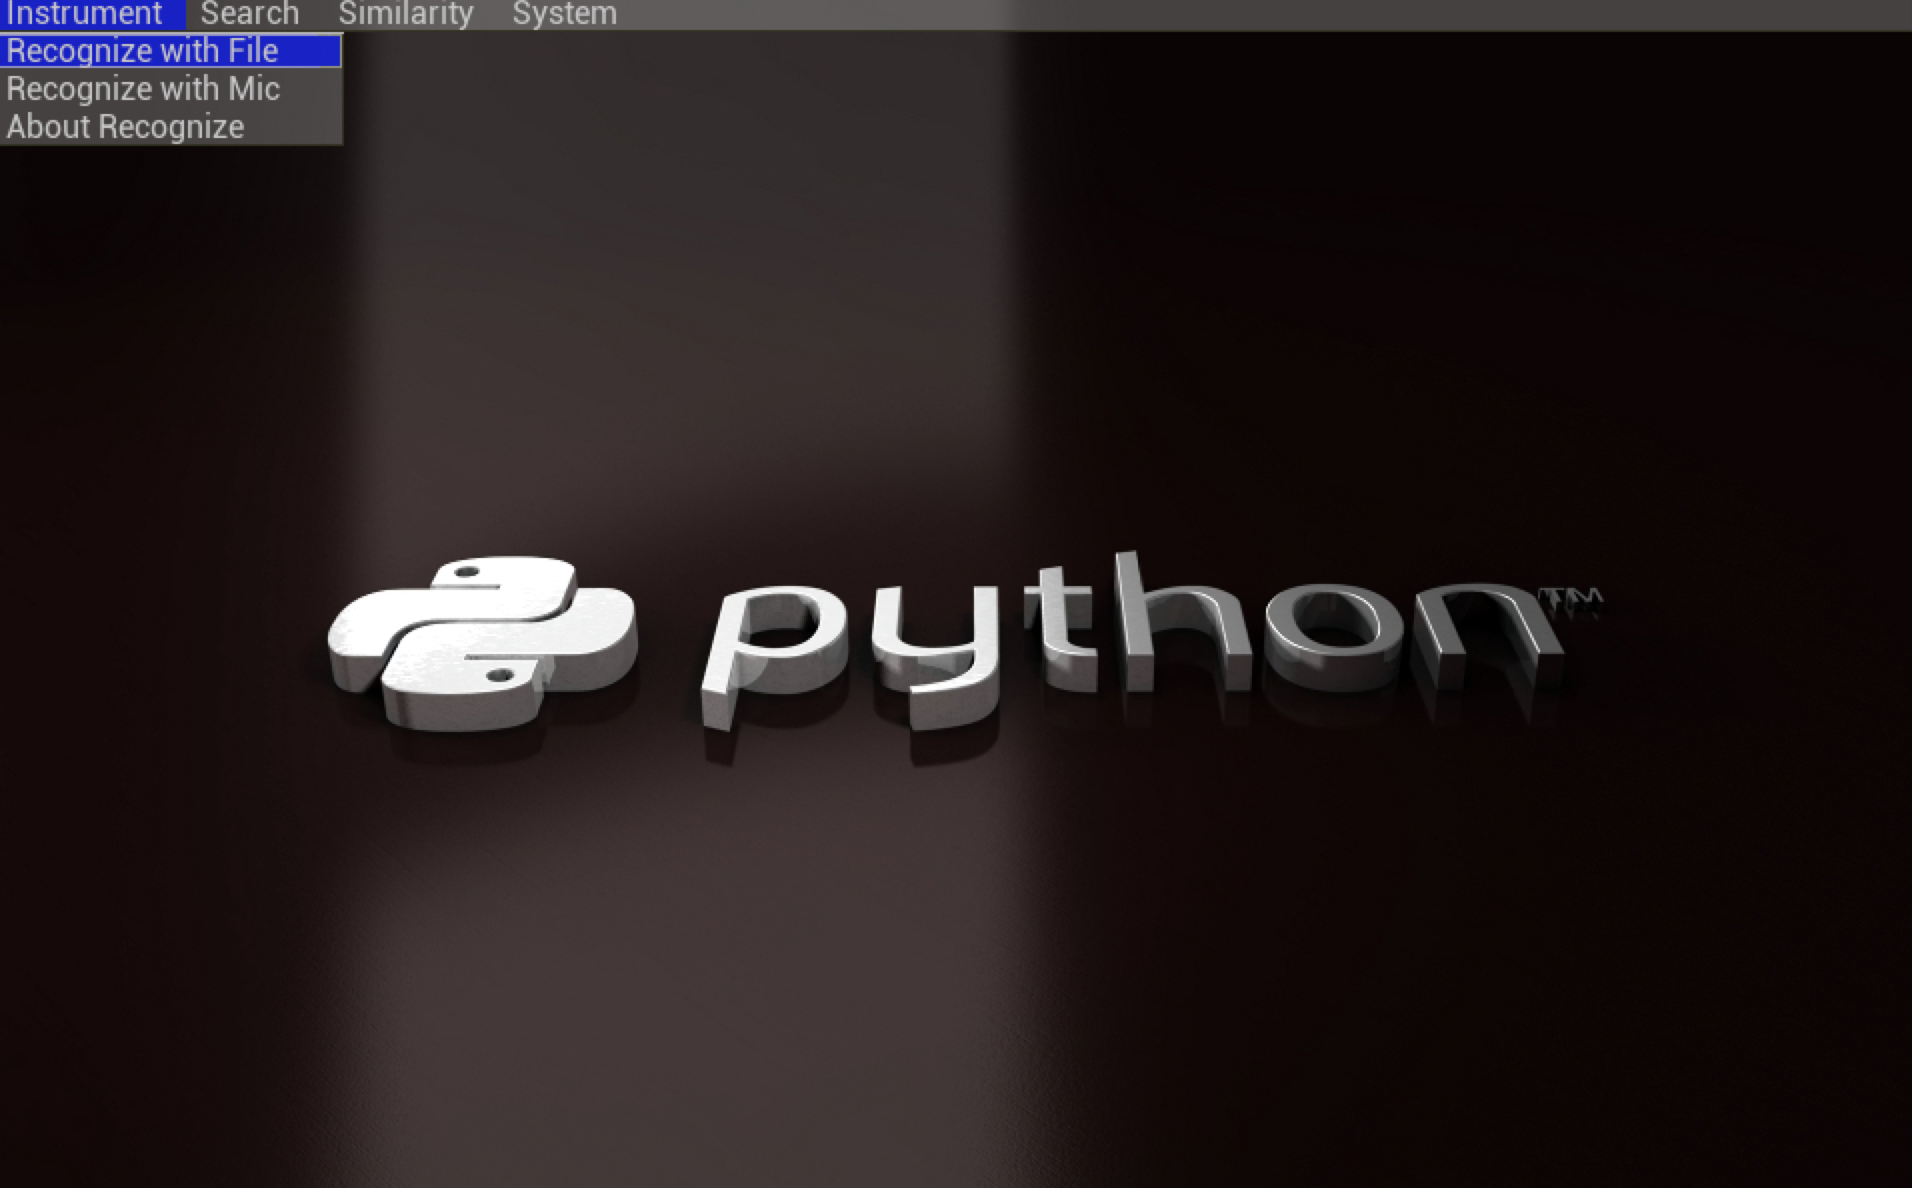
\includegraphics[width=\linewidth]{if1}
\endminipage\hfill
\minipage{0.497\textwidth}
  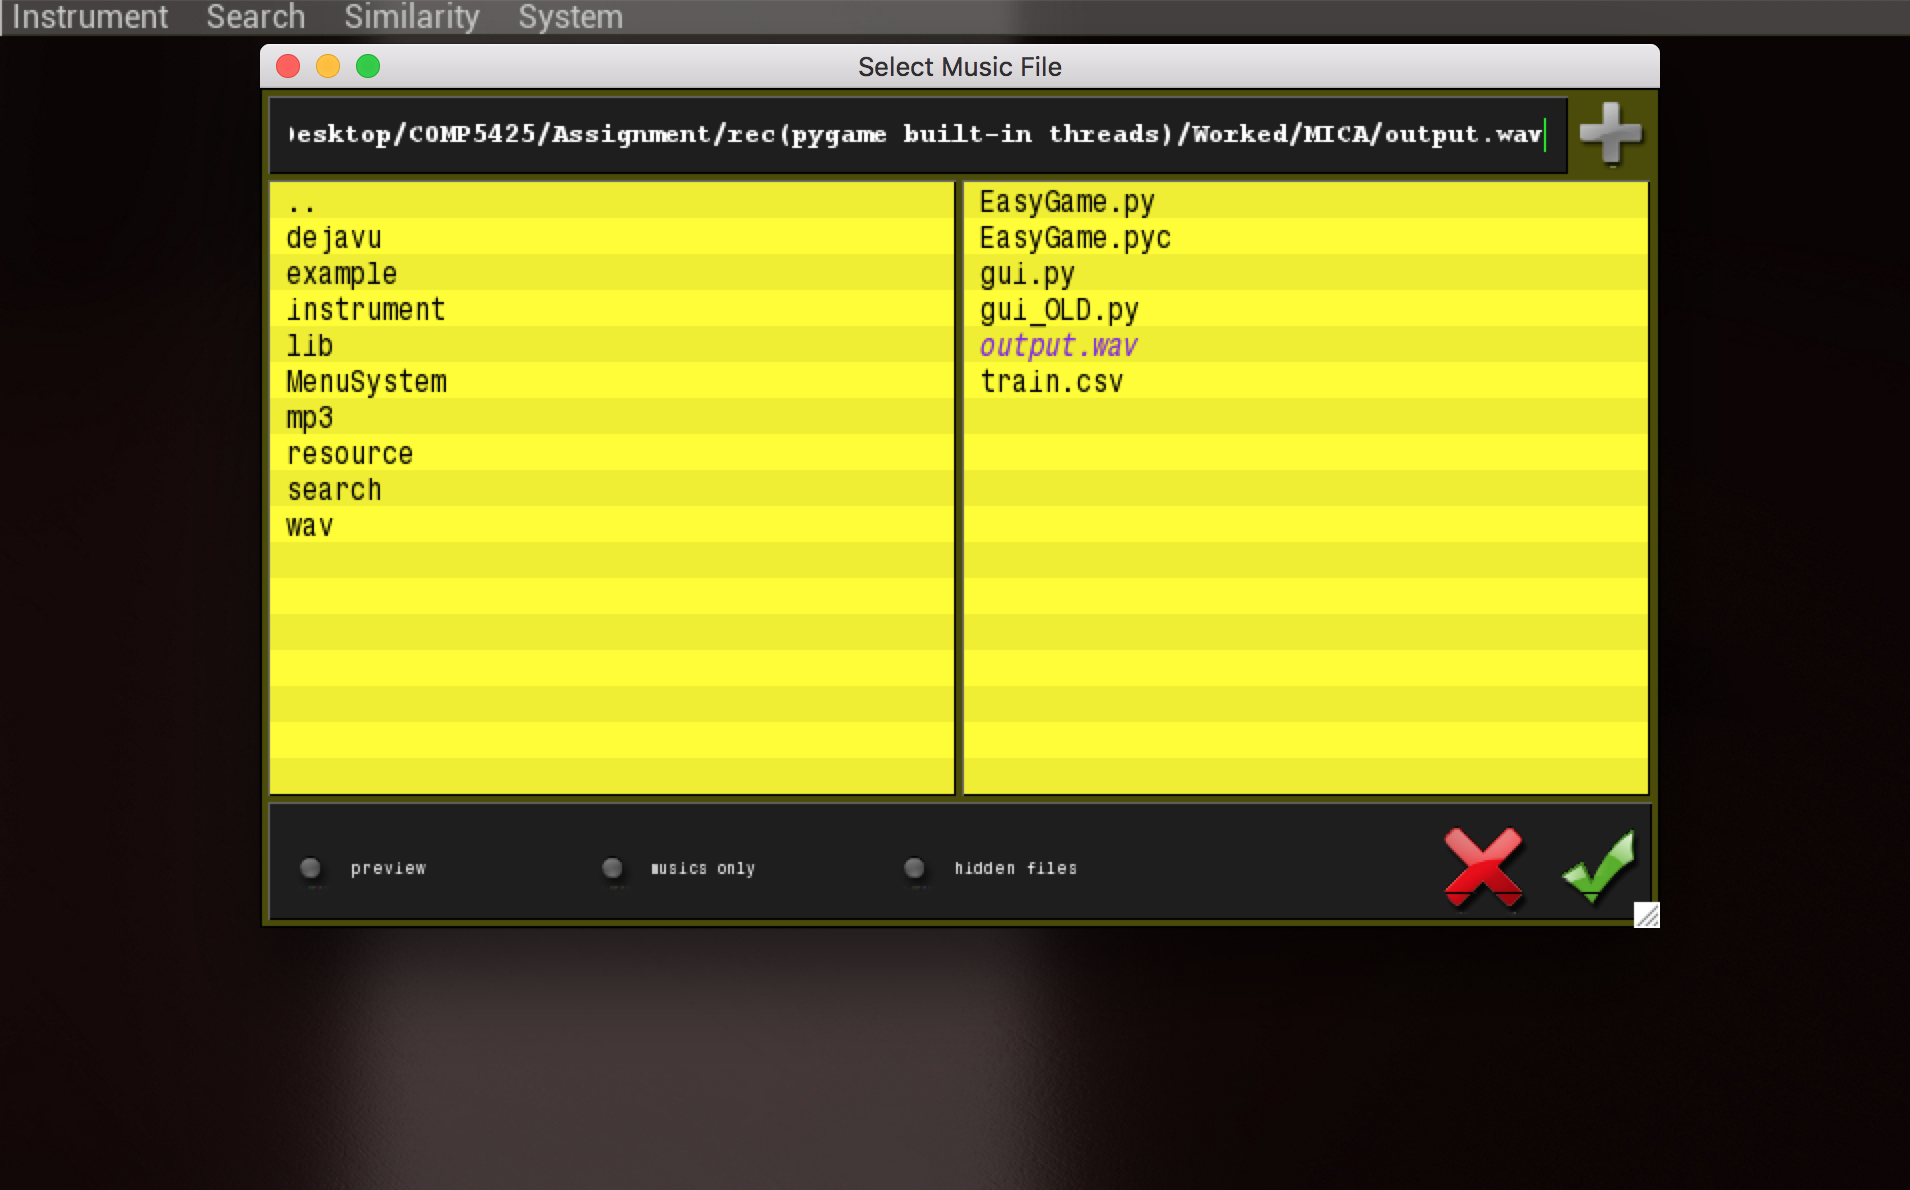
\includegraphics[width=\linewidth]{if2}
  %\caption{A really Awesome Image}\label{fig:awesome_image2}
\endminipage\hfill\\

\minipage{0.497\textwidth}
  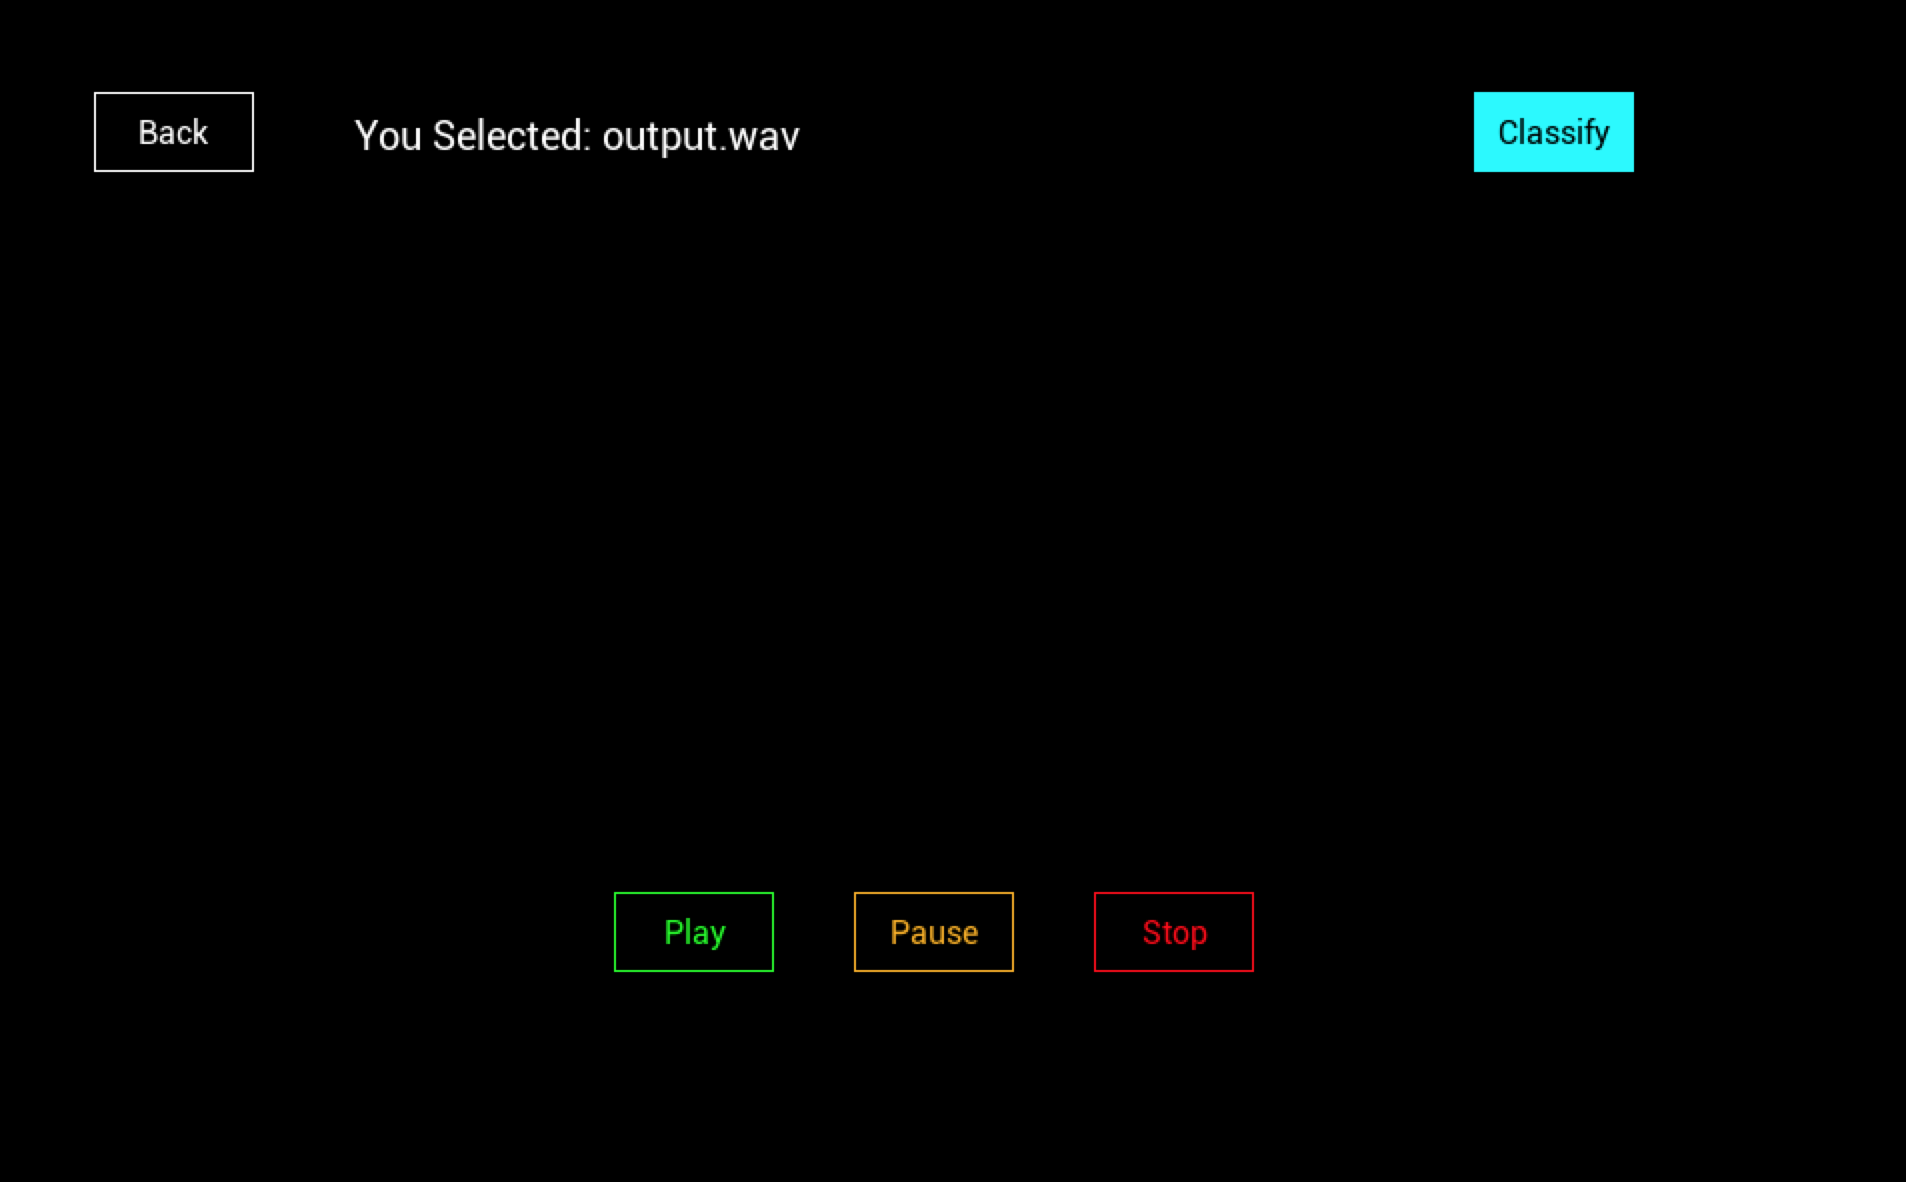
\includegraphics[width=\linewidth]{if3}
  %\caption{A really Awesome Image}\label{fig:awesome_image2}
\endminipage\hfill
\minipage{0.497\textwidth}
  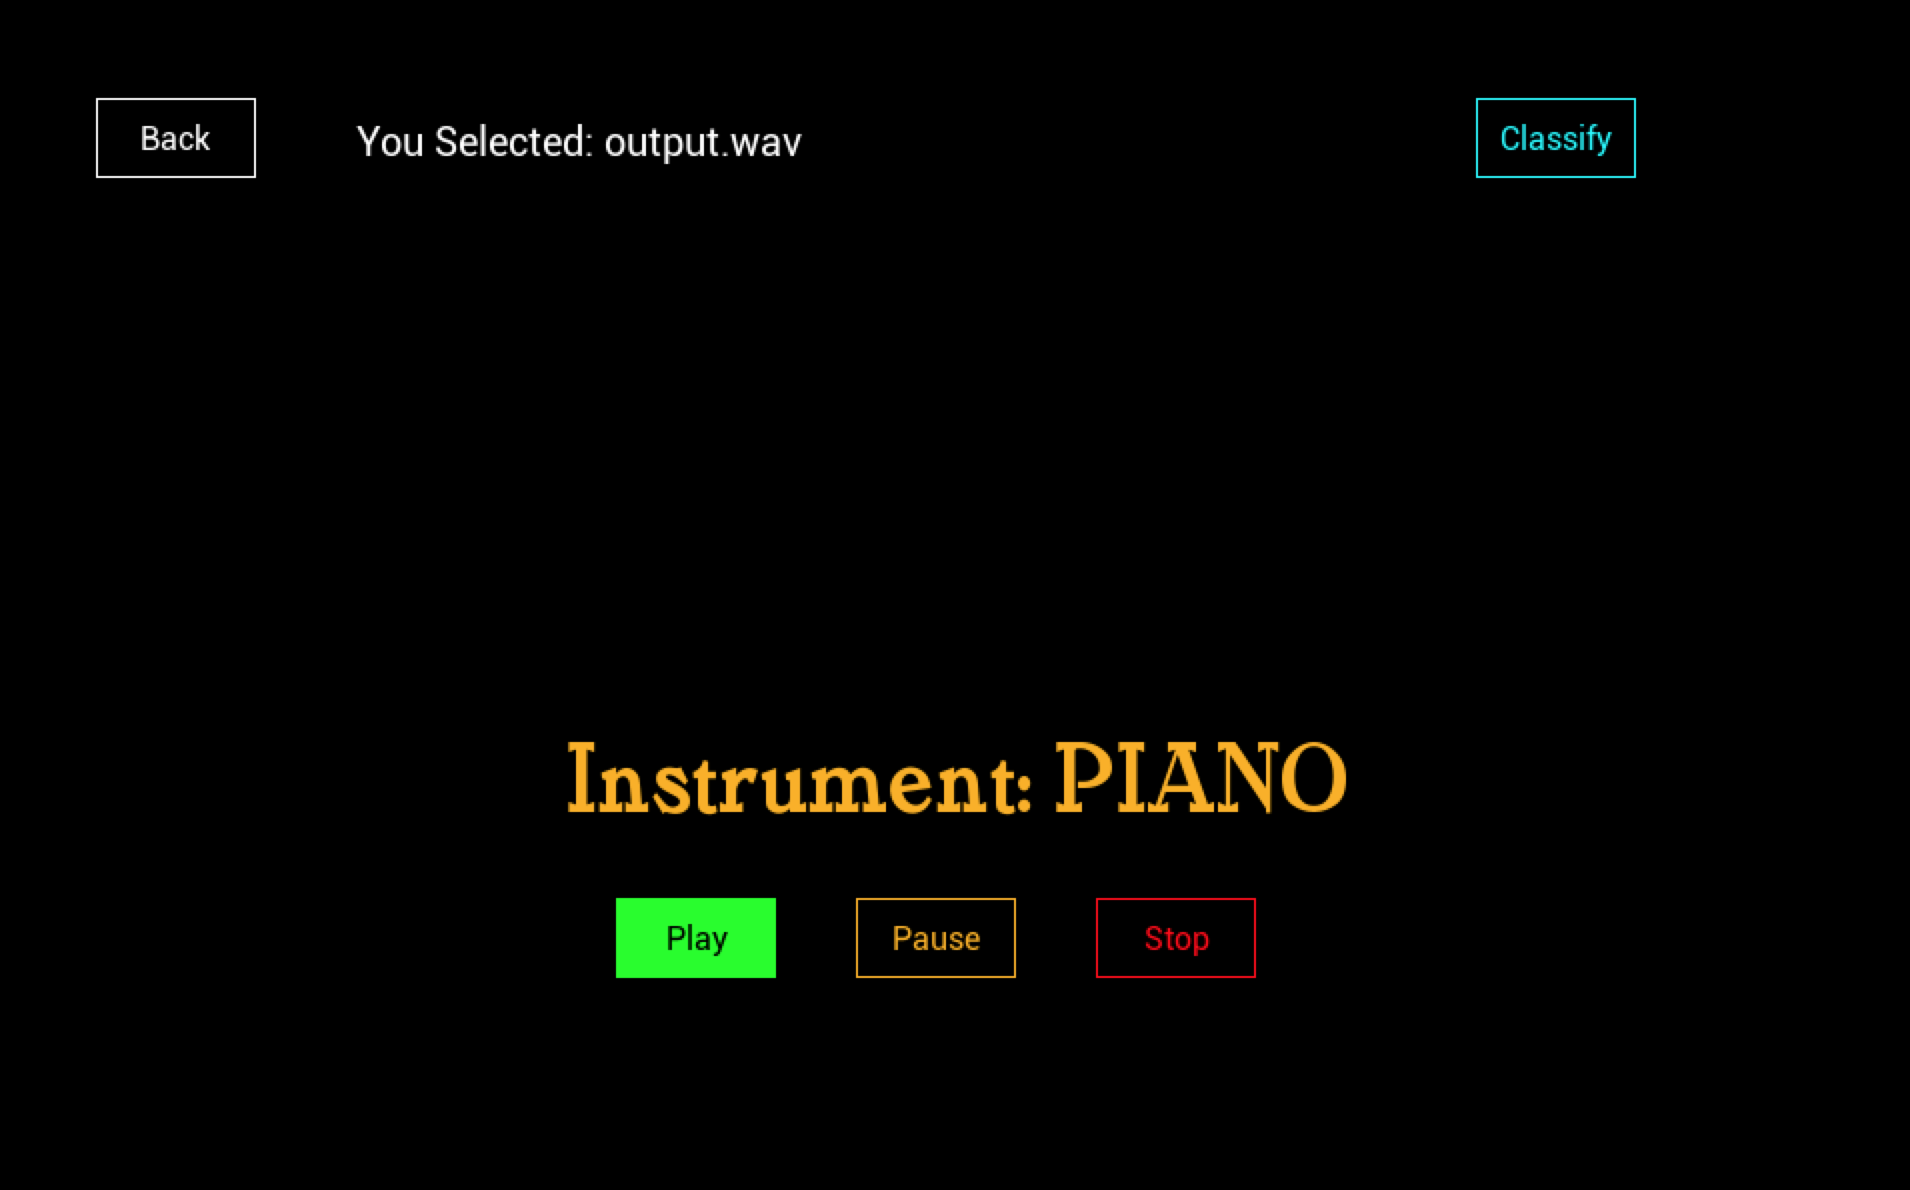
\includegraphics[width=\linewidth]{if4}
  %\caption{A really Awesome Image}\label{fig:awesome_image2}
\endminipage\hfill

\caption{Walk through of Instrument classification by uploading a file. User selects "Instrument by File" in menu, uploads audio file , then clicks on the "Classify" button to reveal played instruments in target audio.}
\label{fig:if}
\end{figure}

\begin{figure}[!htb]
\minipage{0.497\textwidth}
  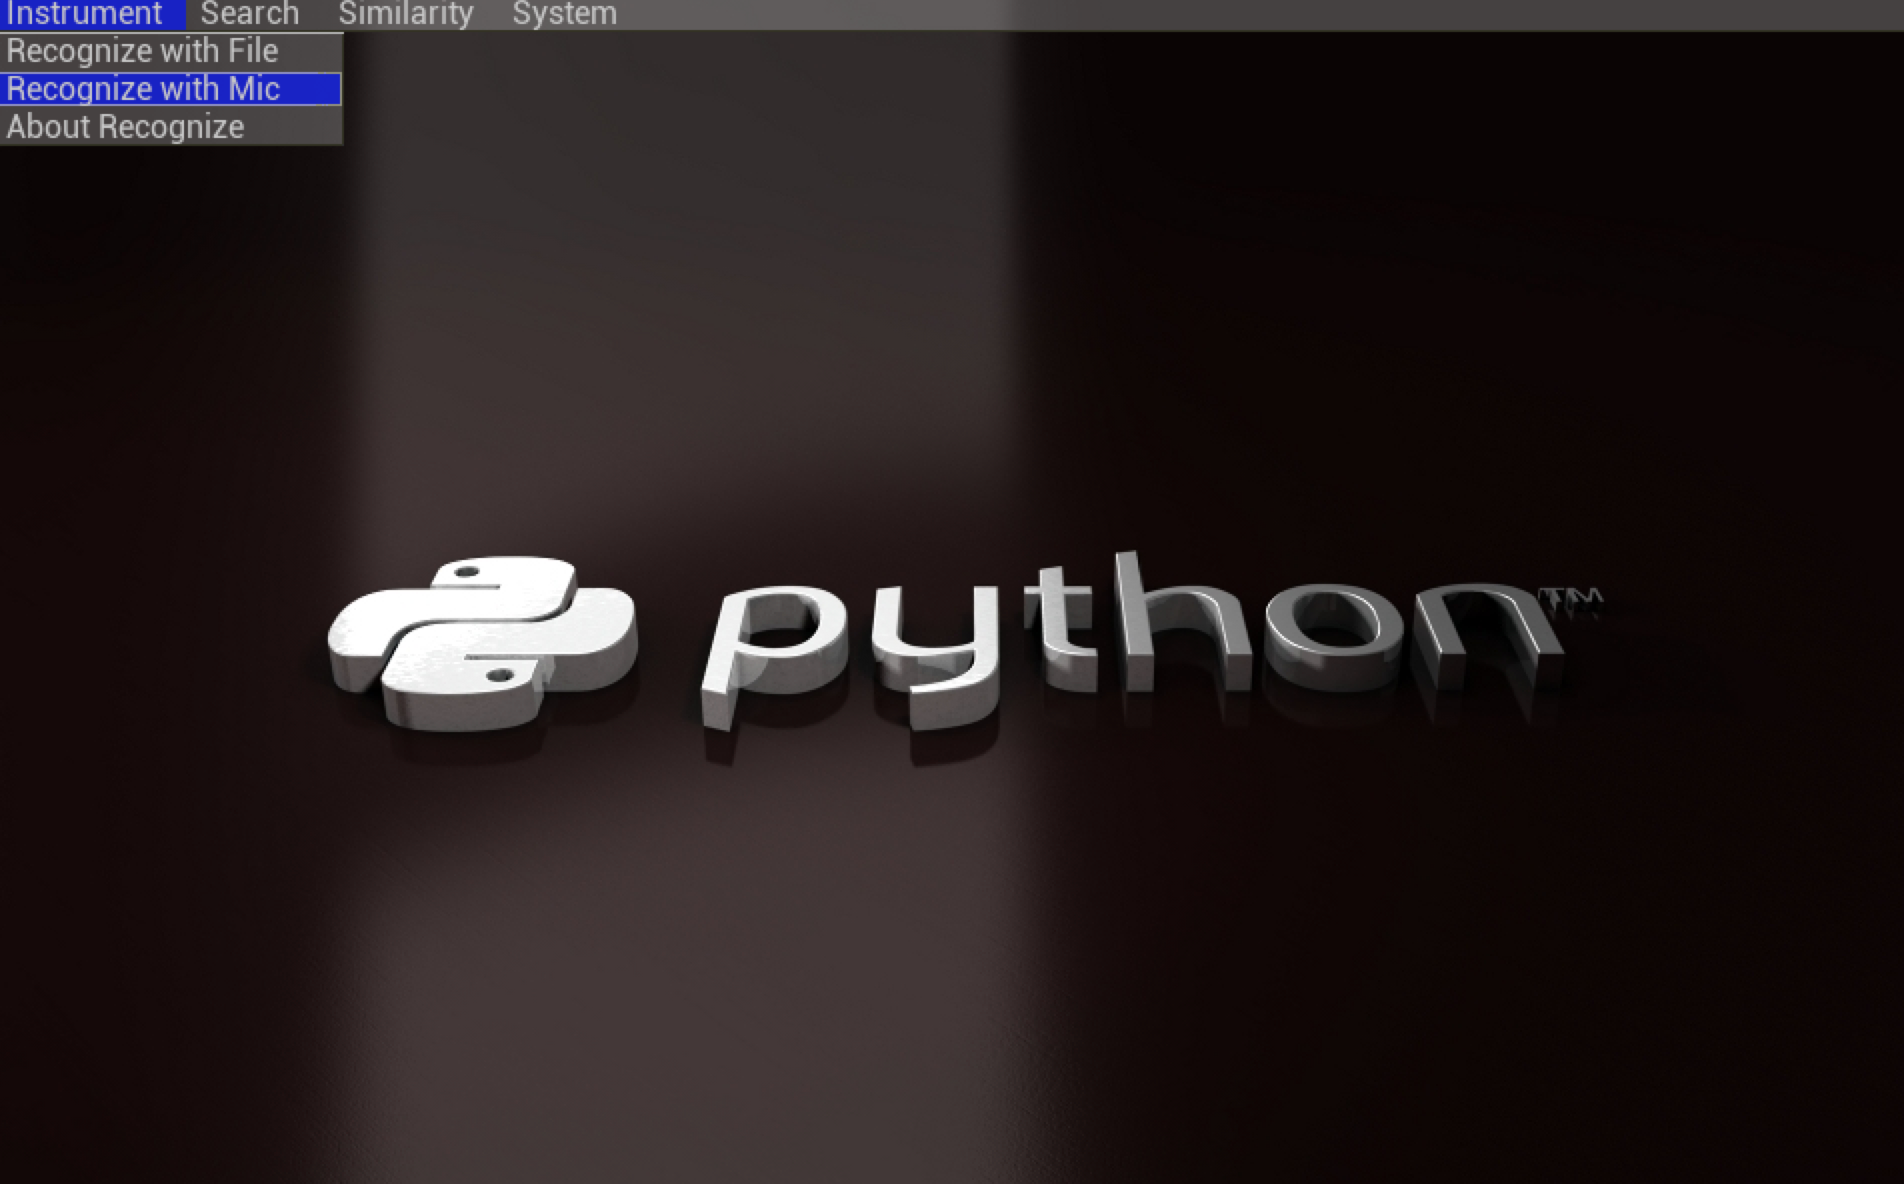
\includegraphics[width=\linewidth]{im1}
\endminipage\hfill
\minipage{0.497\textwidth}
  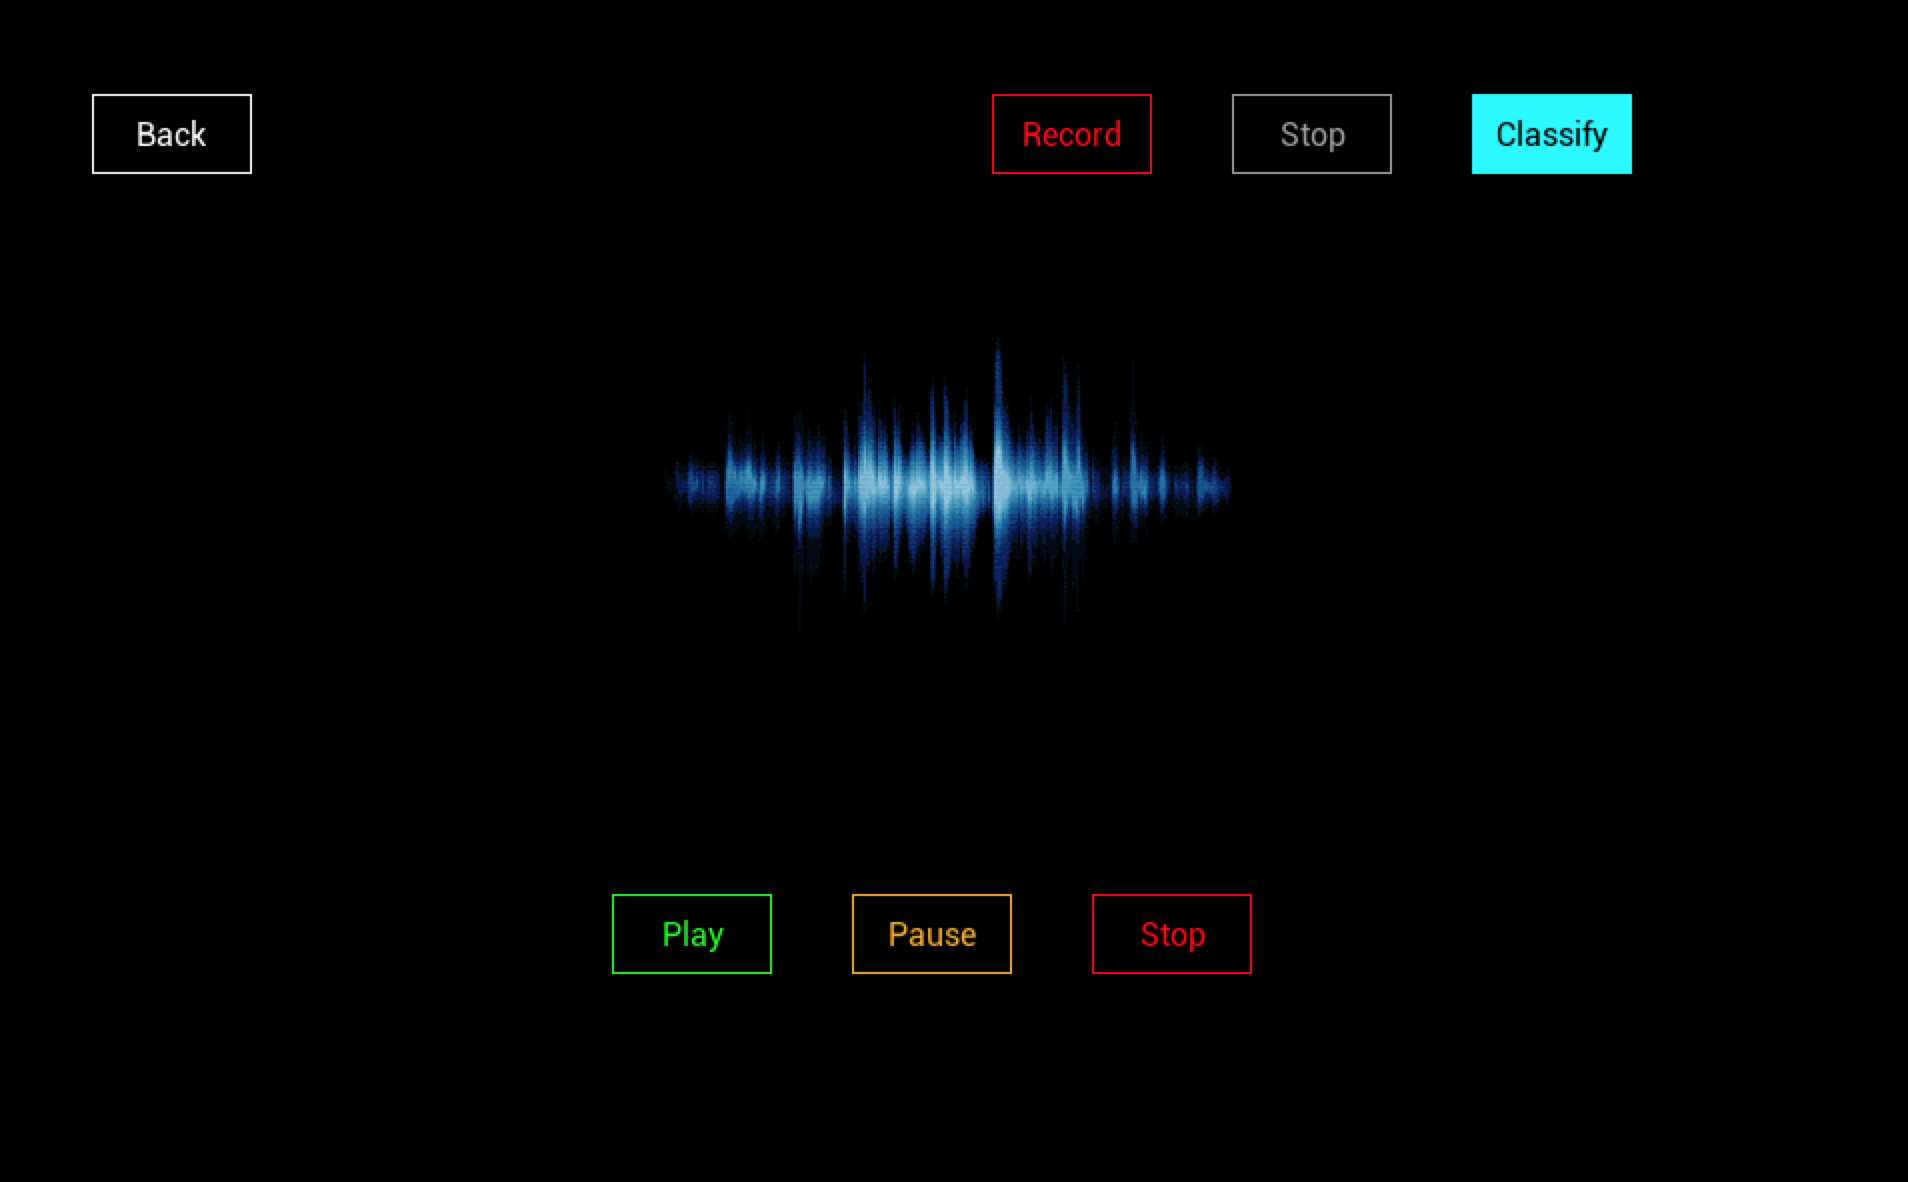
\includegraphics[width=\linewidth]{im2}
  %\caption{A really Awesome Image}\label{fig:awesome_image2}
\endminipage\hfill\\

\minipage{0.497\textwidth}
  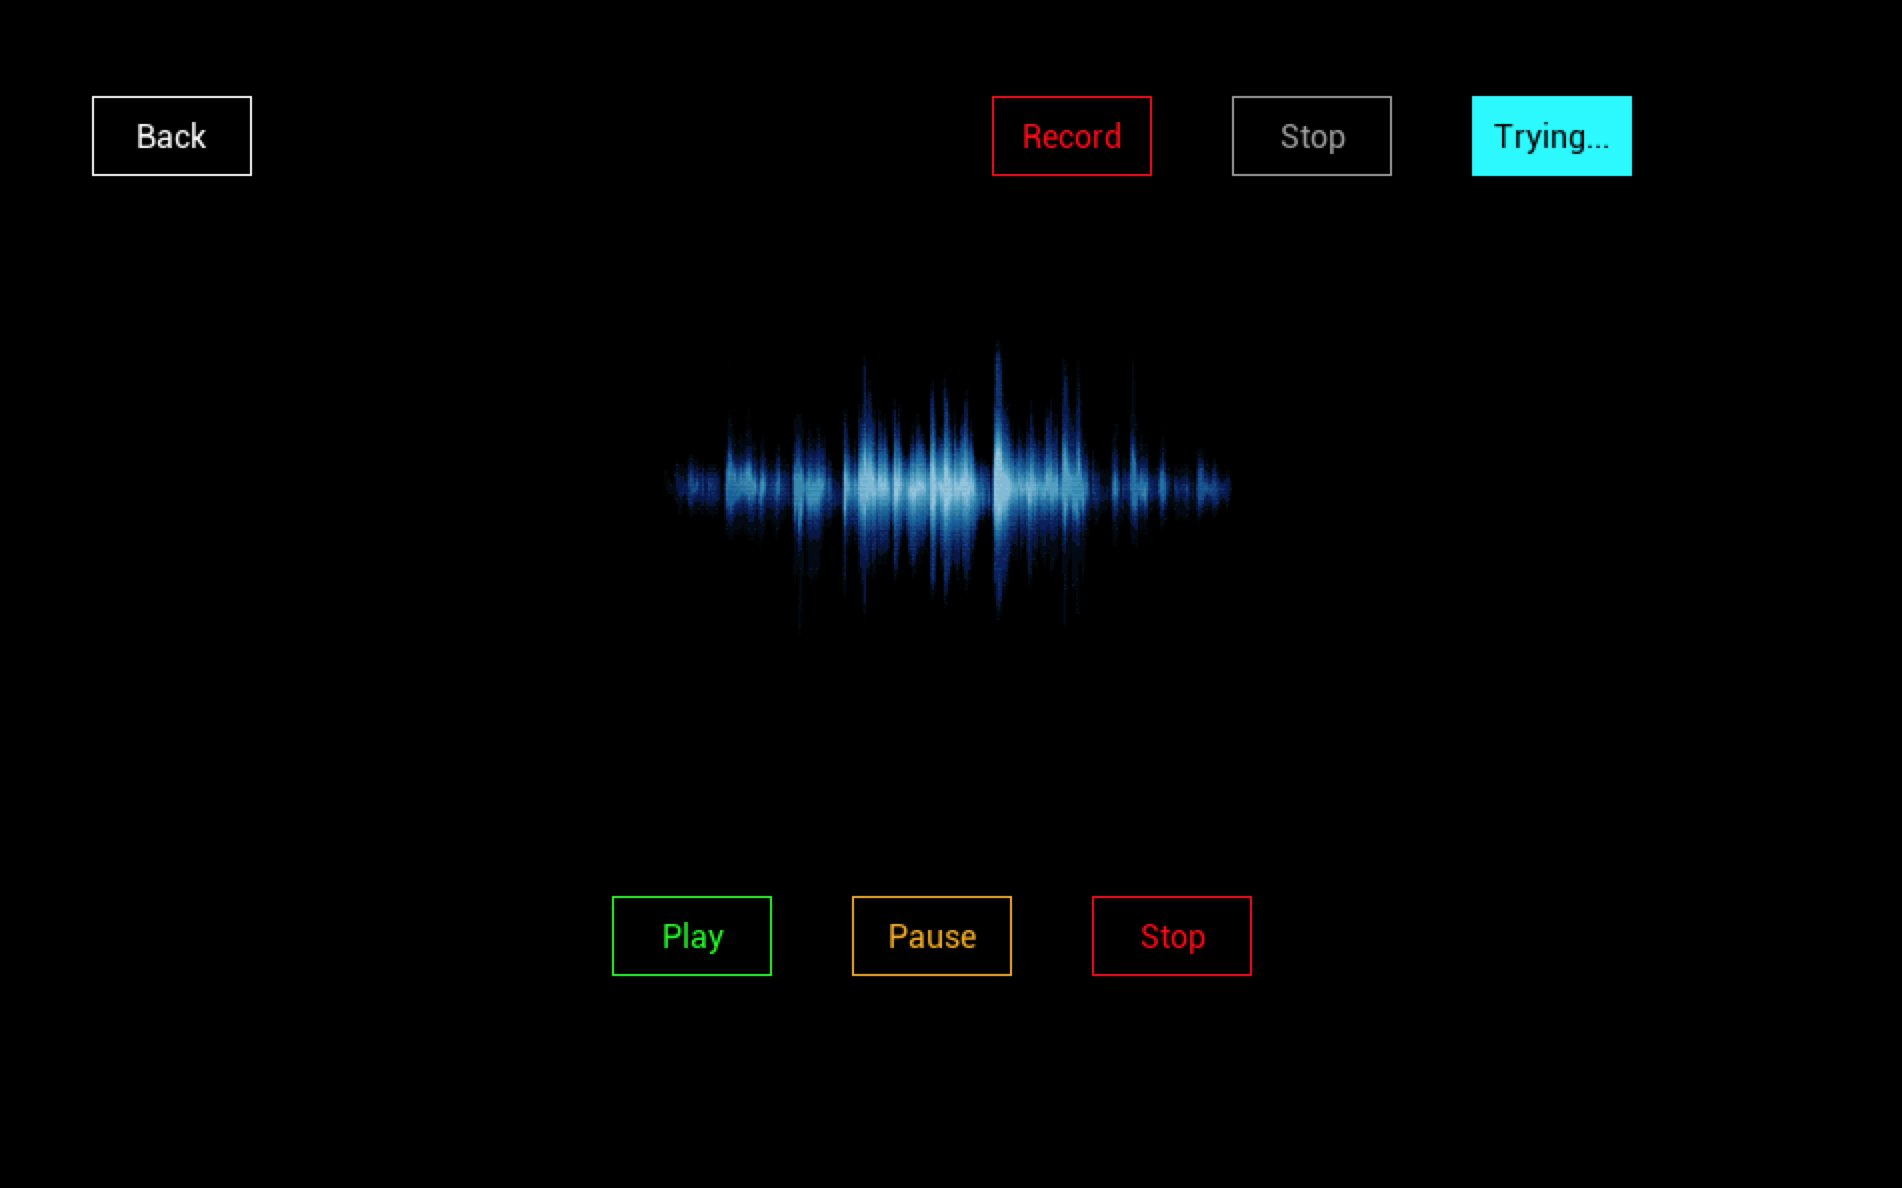
\includegraphics[width=\linewidth]{im3}
  %\caption{A really Awesome Image}\label{fig:awesome_image2}
\endminipage\hfill
\minipage{0.497\textwidth}
  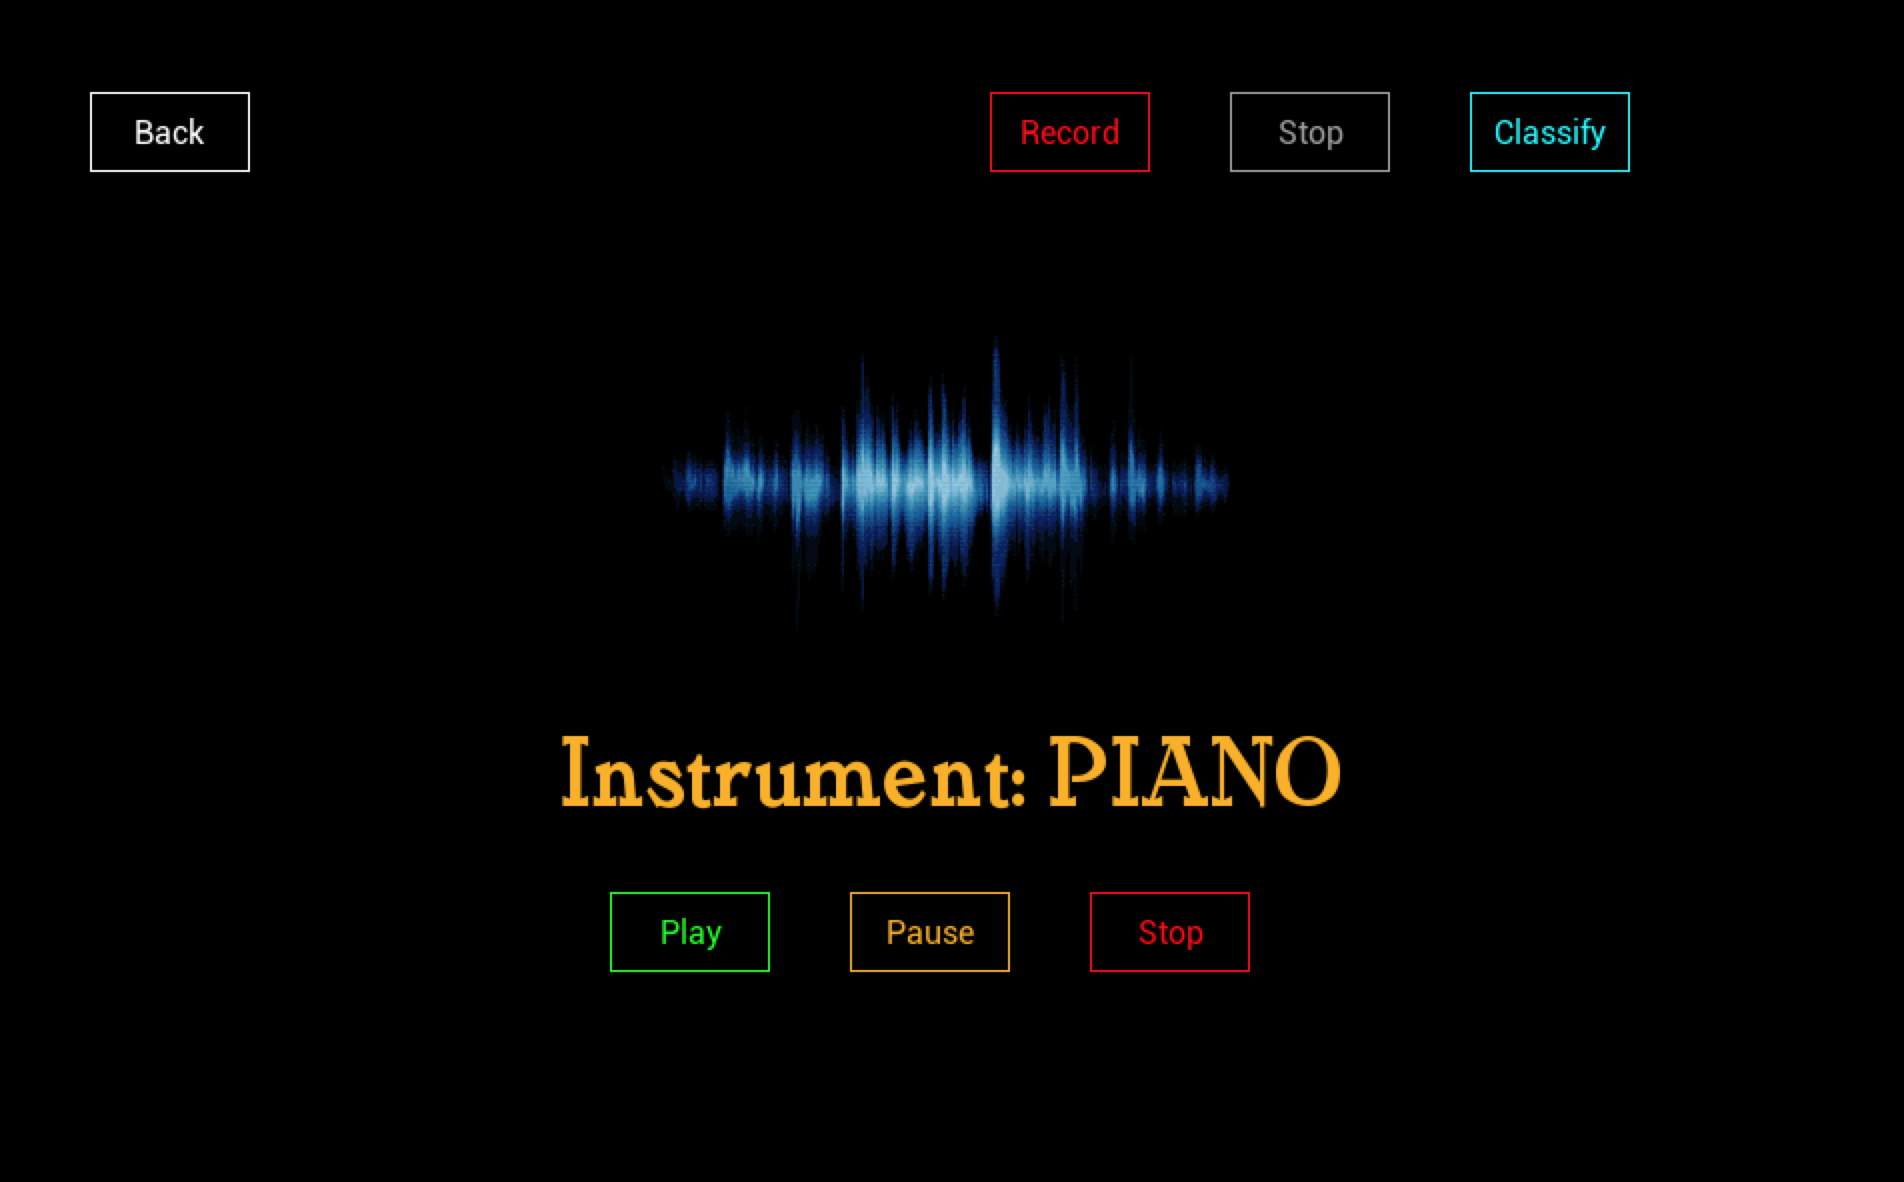
\includegraphics[width=\linewidth]{im4}
  %\caption{A really Awesome Image}\label{fig:awesome_image2}
\endminipage\hfill

\caption{Walk through of Instrument classification through microphone. User selects "Instrument by Mic" in menu, records a clip of  audio, then clicks on the "Classify" button to reveal played instruments in target audio.}
\label{fig:im}
\end{figure}

\section{Searching}
Audio fingerprint is generated using a audio fingerprinting and recognition algorithm implemented in $dejavu$\footnote{\url{https://github.com/worldveil/dejavu}}, which can memorize audios by listening to it once and fingerprinting it. Then using resulting fingerprints to match input audio against our database (using $mysql$\footnote{\url{https://www.mysql.com}}).

\subsection{Storyboard Walk Through}
The walk through for  using searching function is shown in Figure~\ref{fig:sf} and~\ref{fig:sm} from left to right, top to bottom.

\begin{figure}[!htb]
\minipage{0.497\textwidth}
  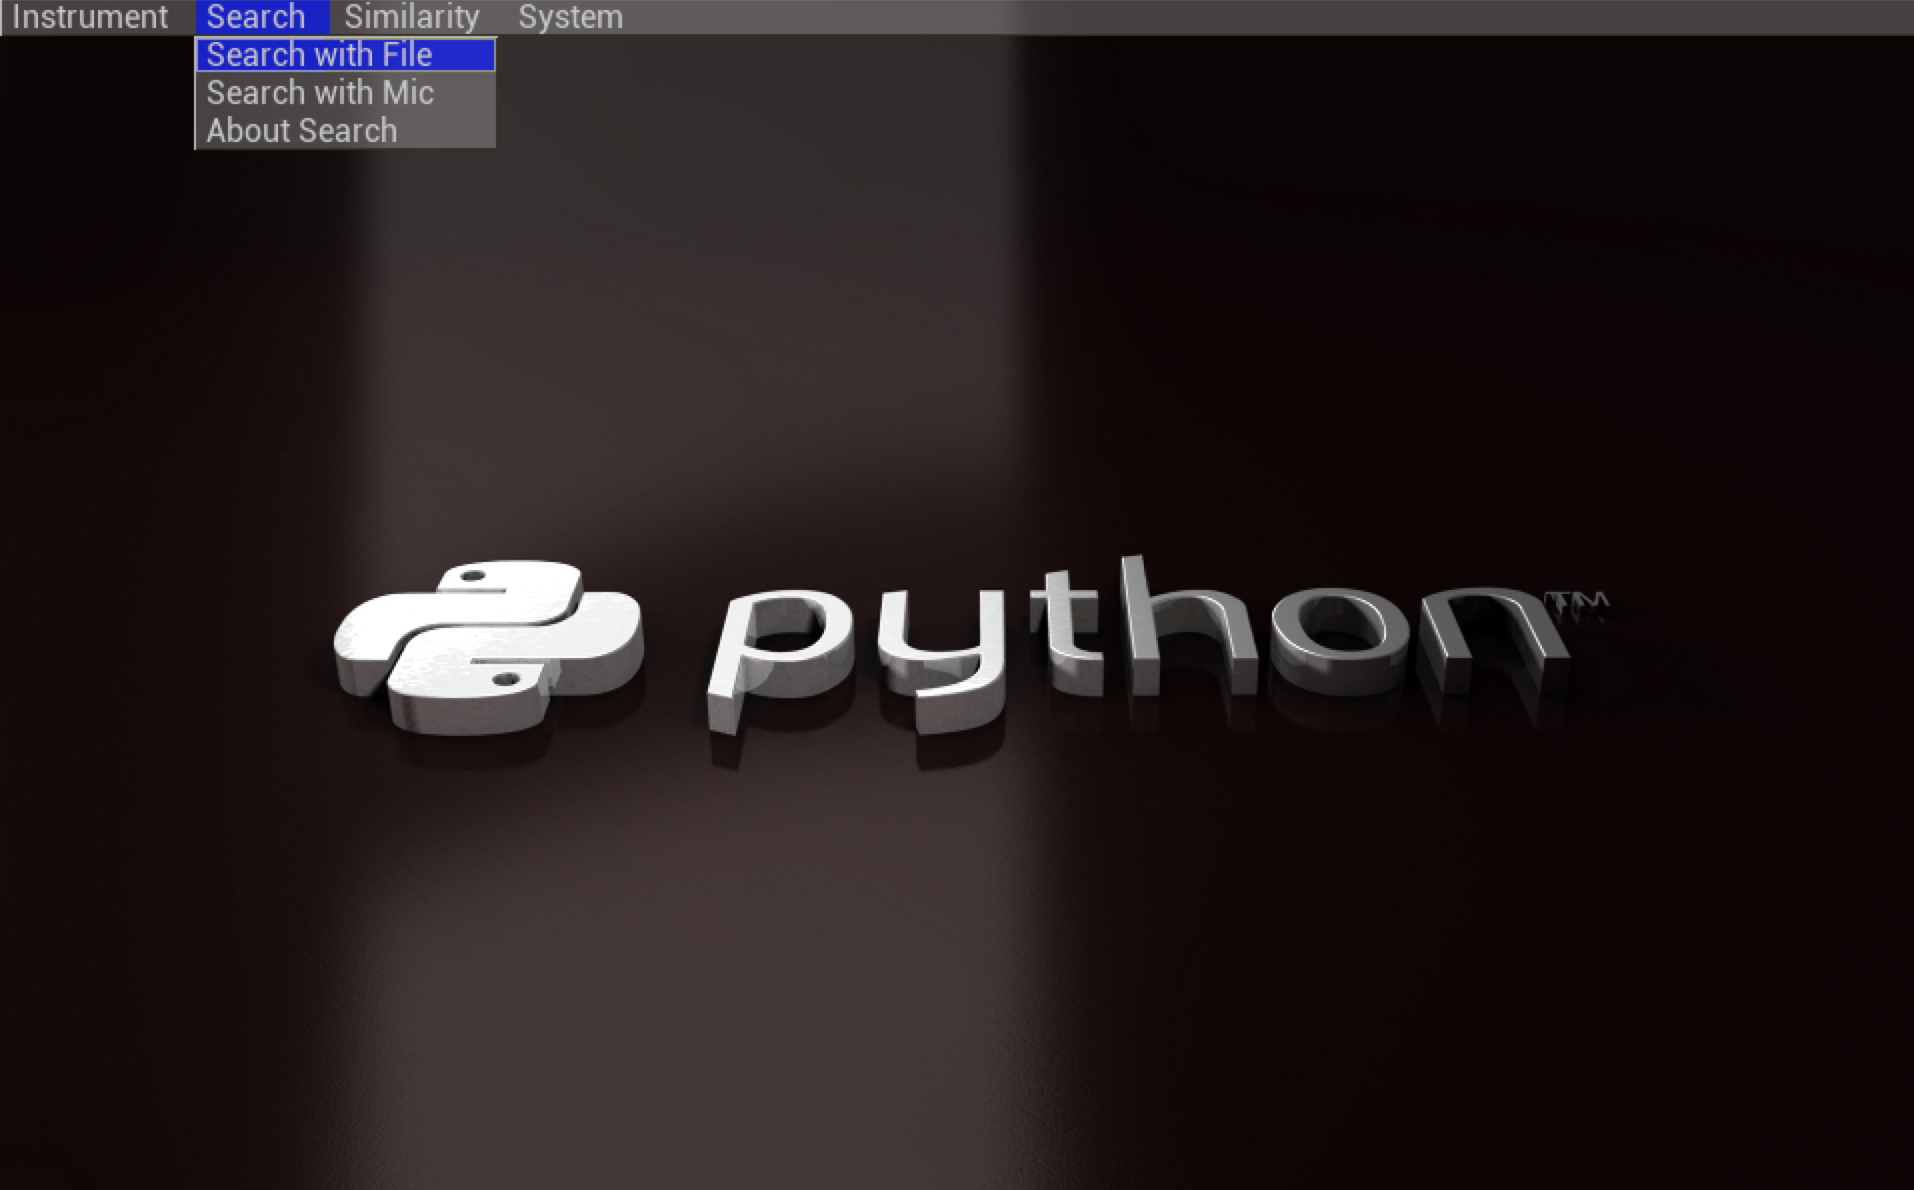
\includegraphics[width=\linewidth]{sf1}
\endminipage\hfill
\minipage{0.497\textwidth}
  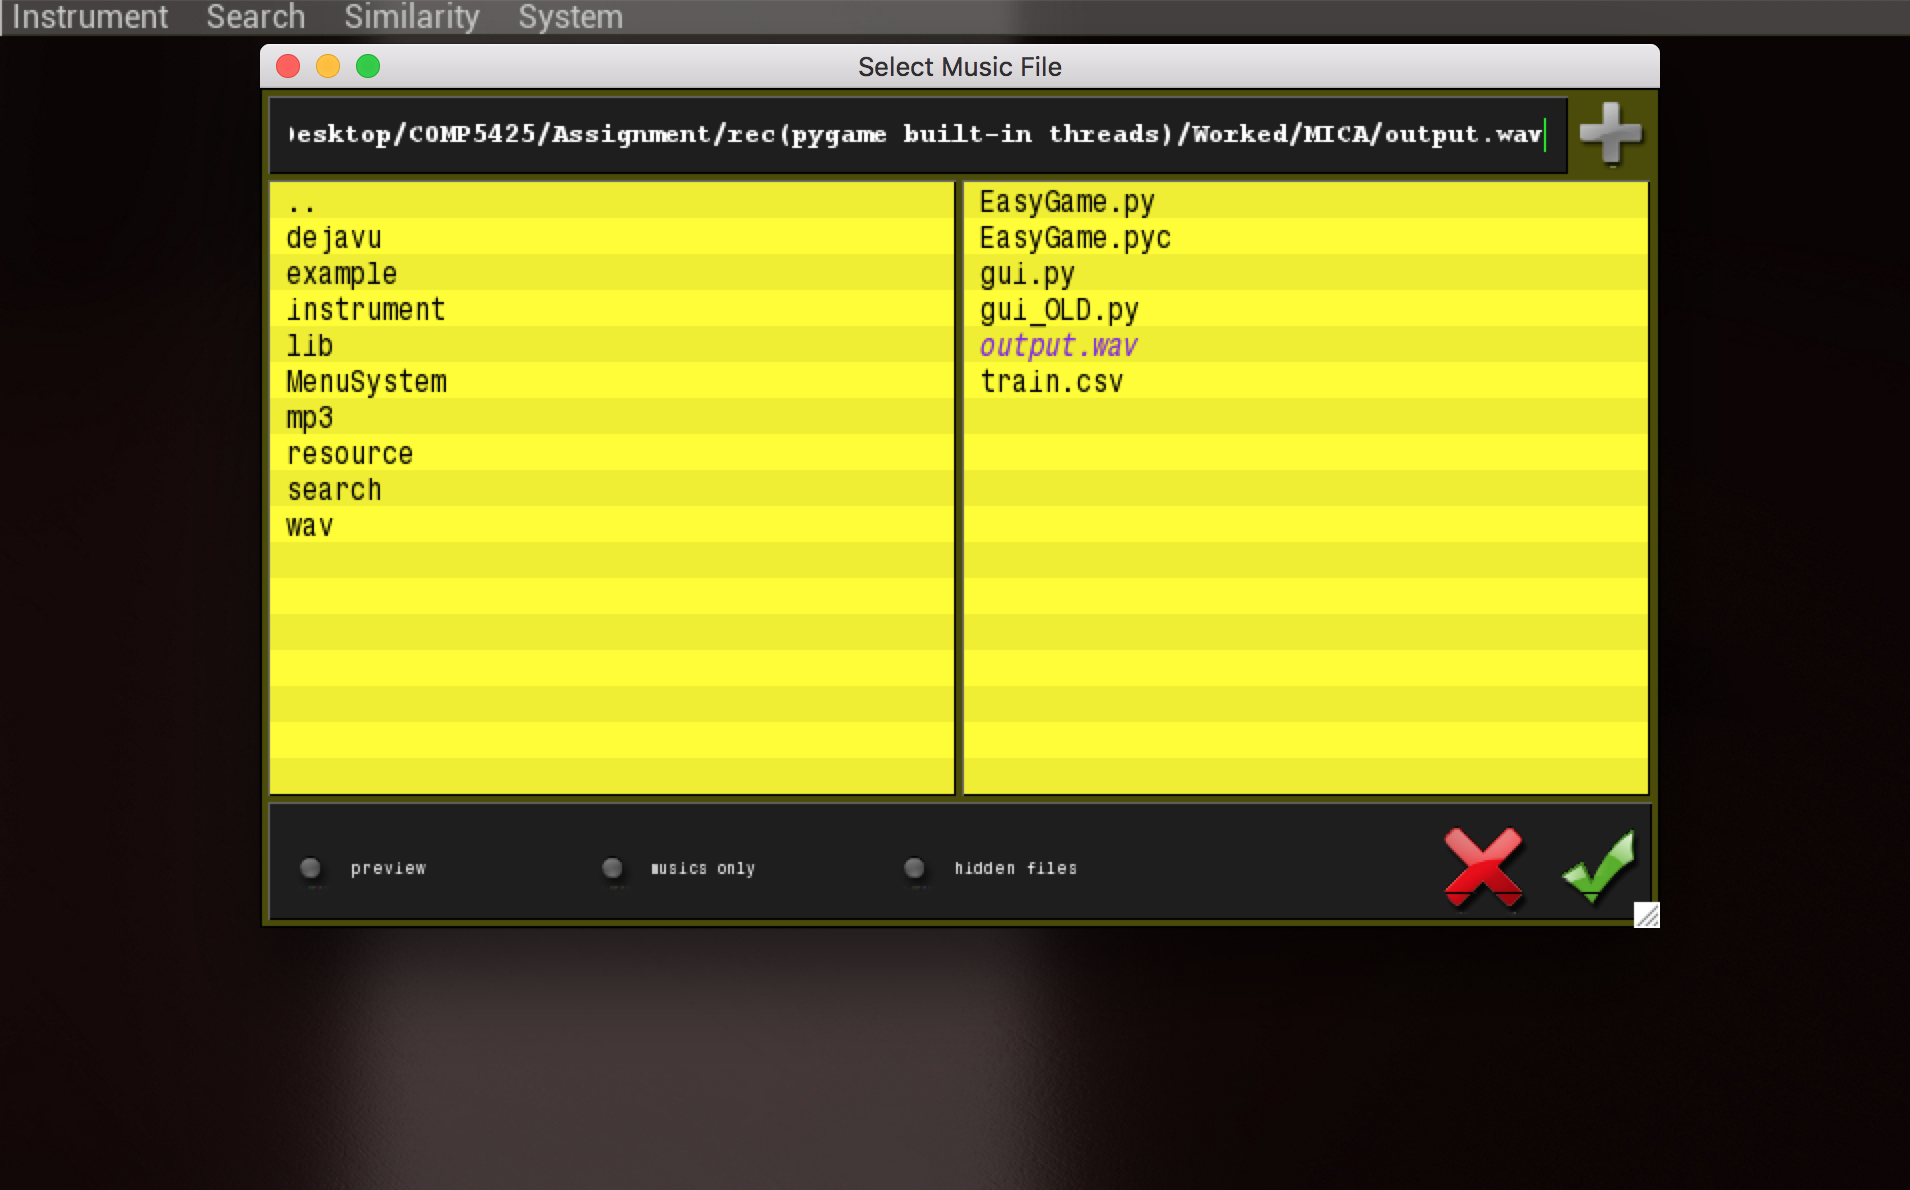
\includegraphics[width=\linewidth]{if2}
  %\caption{A really Awesome Image}\label{fig:awesome_image2}
\endminipage\hfill\\

\minipage{0.497\textwidth}
  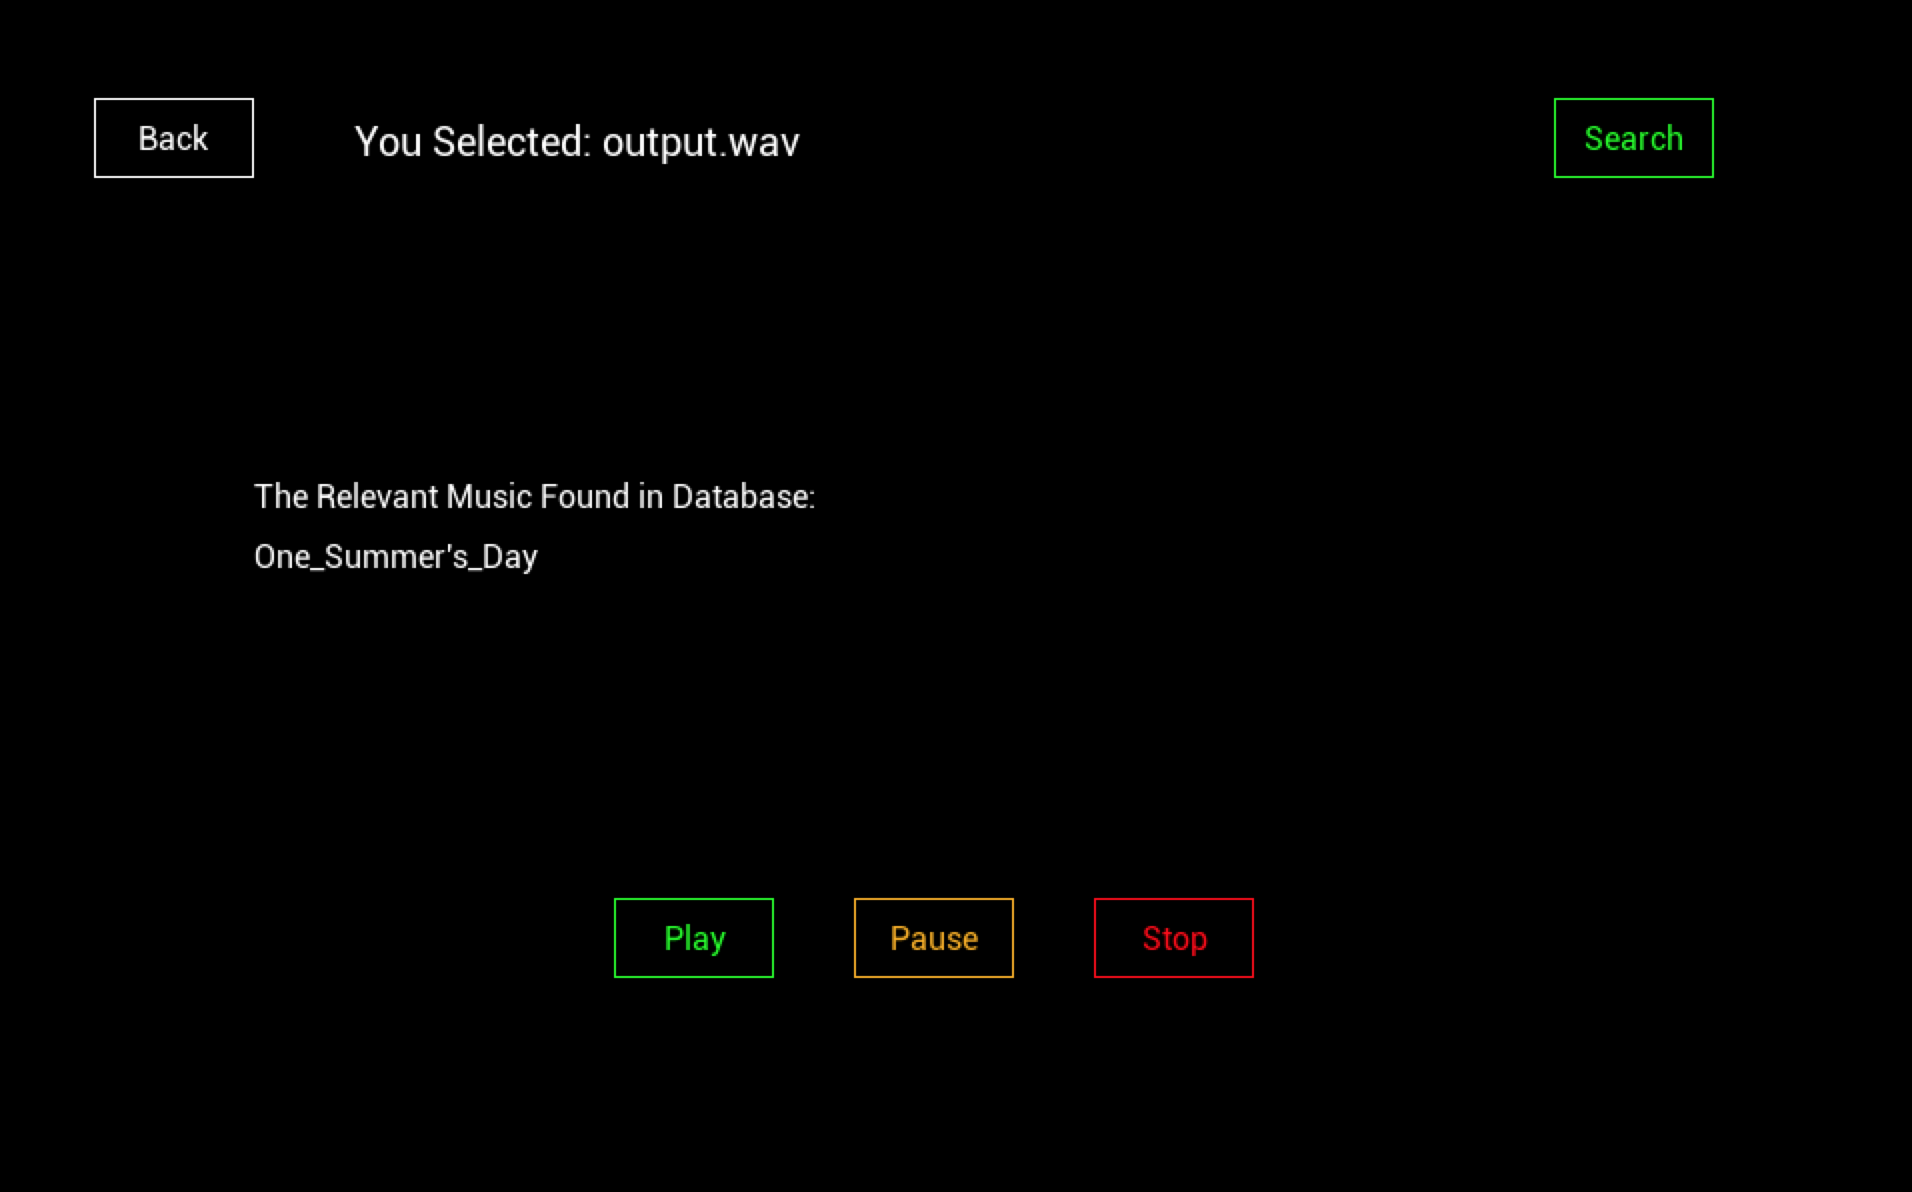
\includegraphics[width=\linewidth]{sf3}
  %\caption{A really Awesome Image}\label{fig:awesome_image2}
\endminipage\hfill
\minipage{0.497\textwidth}
  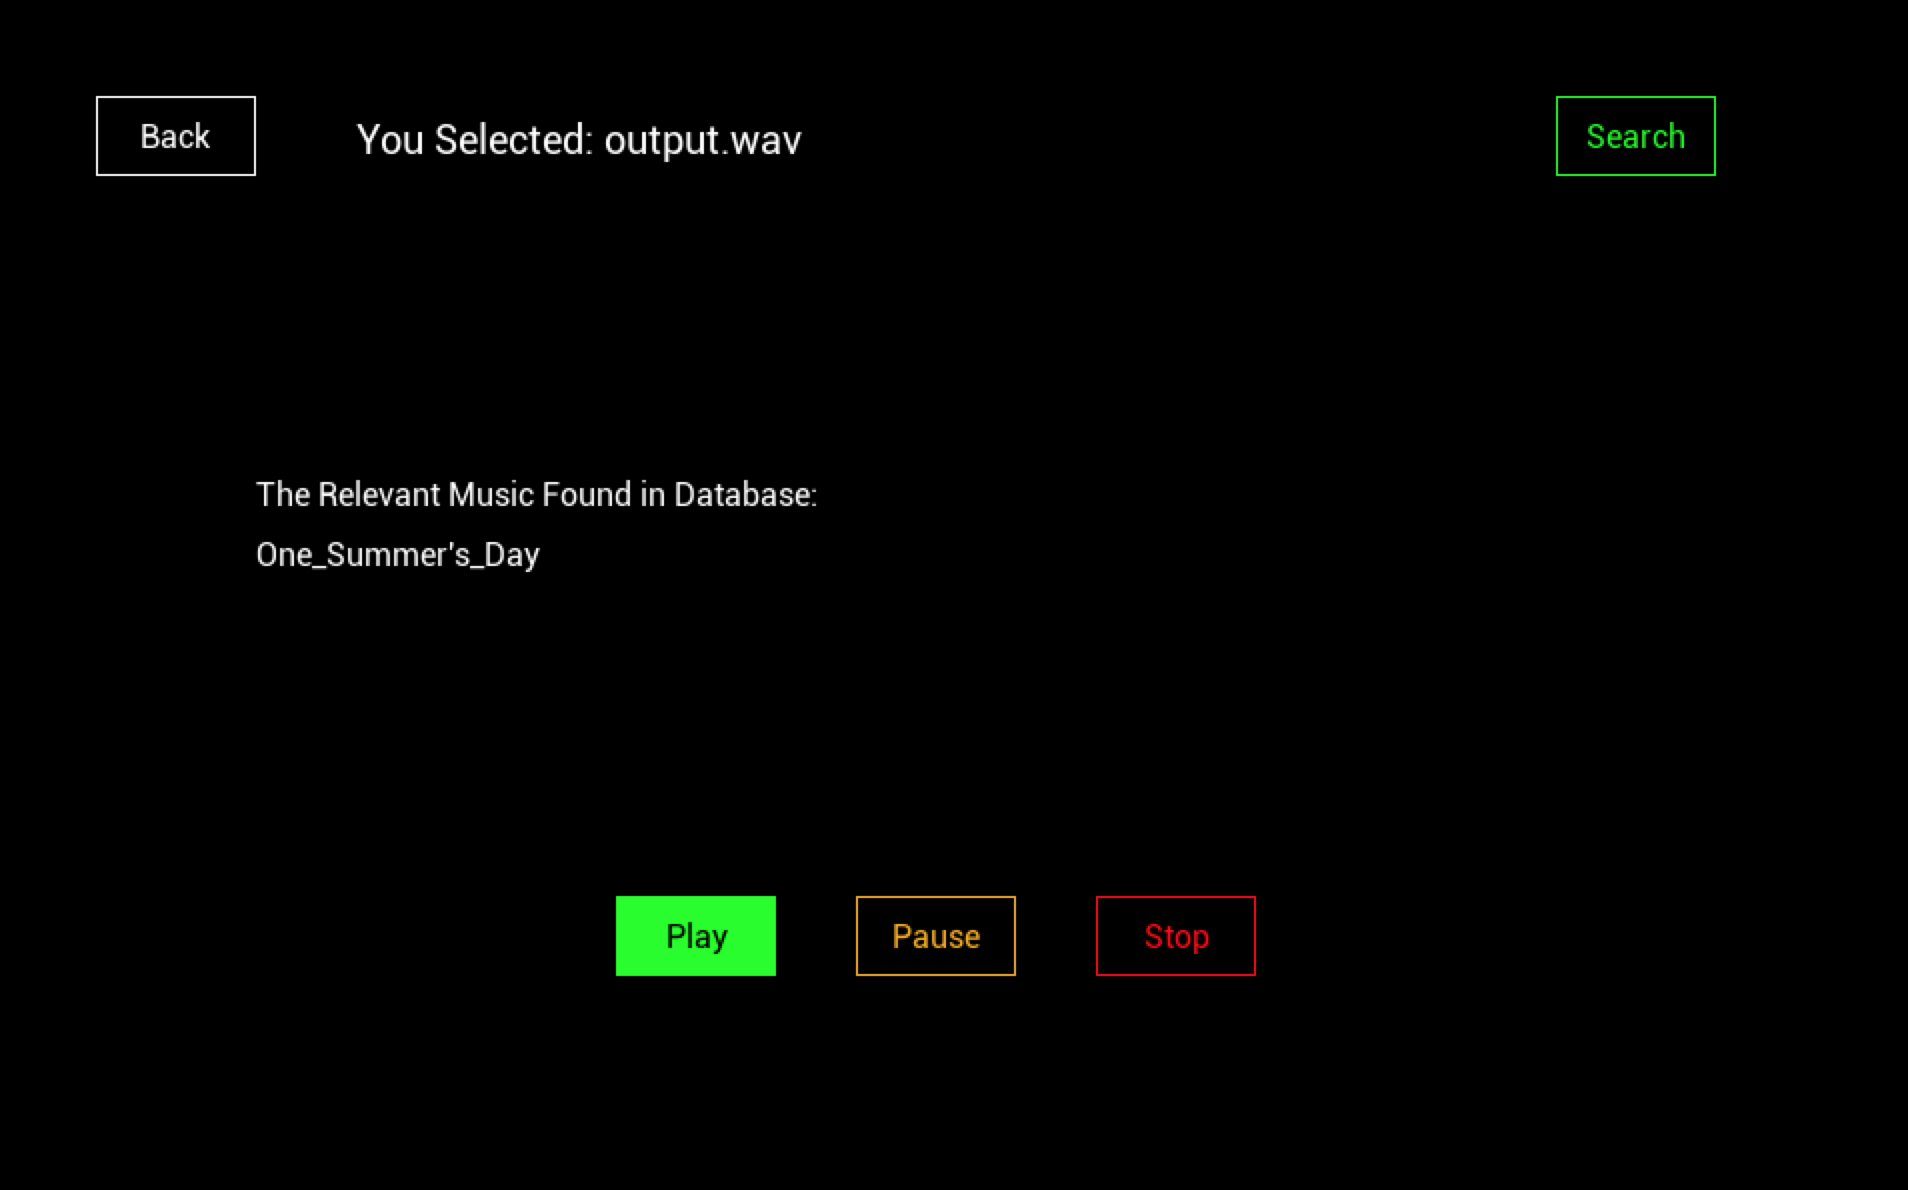
\includegraphics[width=\linewidth]{sf4}
  %\caption{A really Awesome Image}\label{fig:awesome_image2}
\endminipage\hfill

\caption{Walk through of Searching function by uploading a file. User selects "Search by File" in menu, uploads a unknown audio, then click on the "Search" button to reveal matching audio.}
\label{fig:sf}
\end{figure}

\begin{figure}[!htb]
\minipage{0.497\textwidth}
  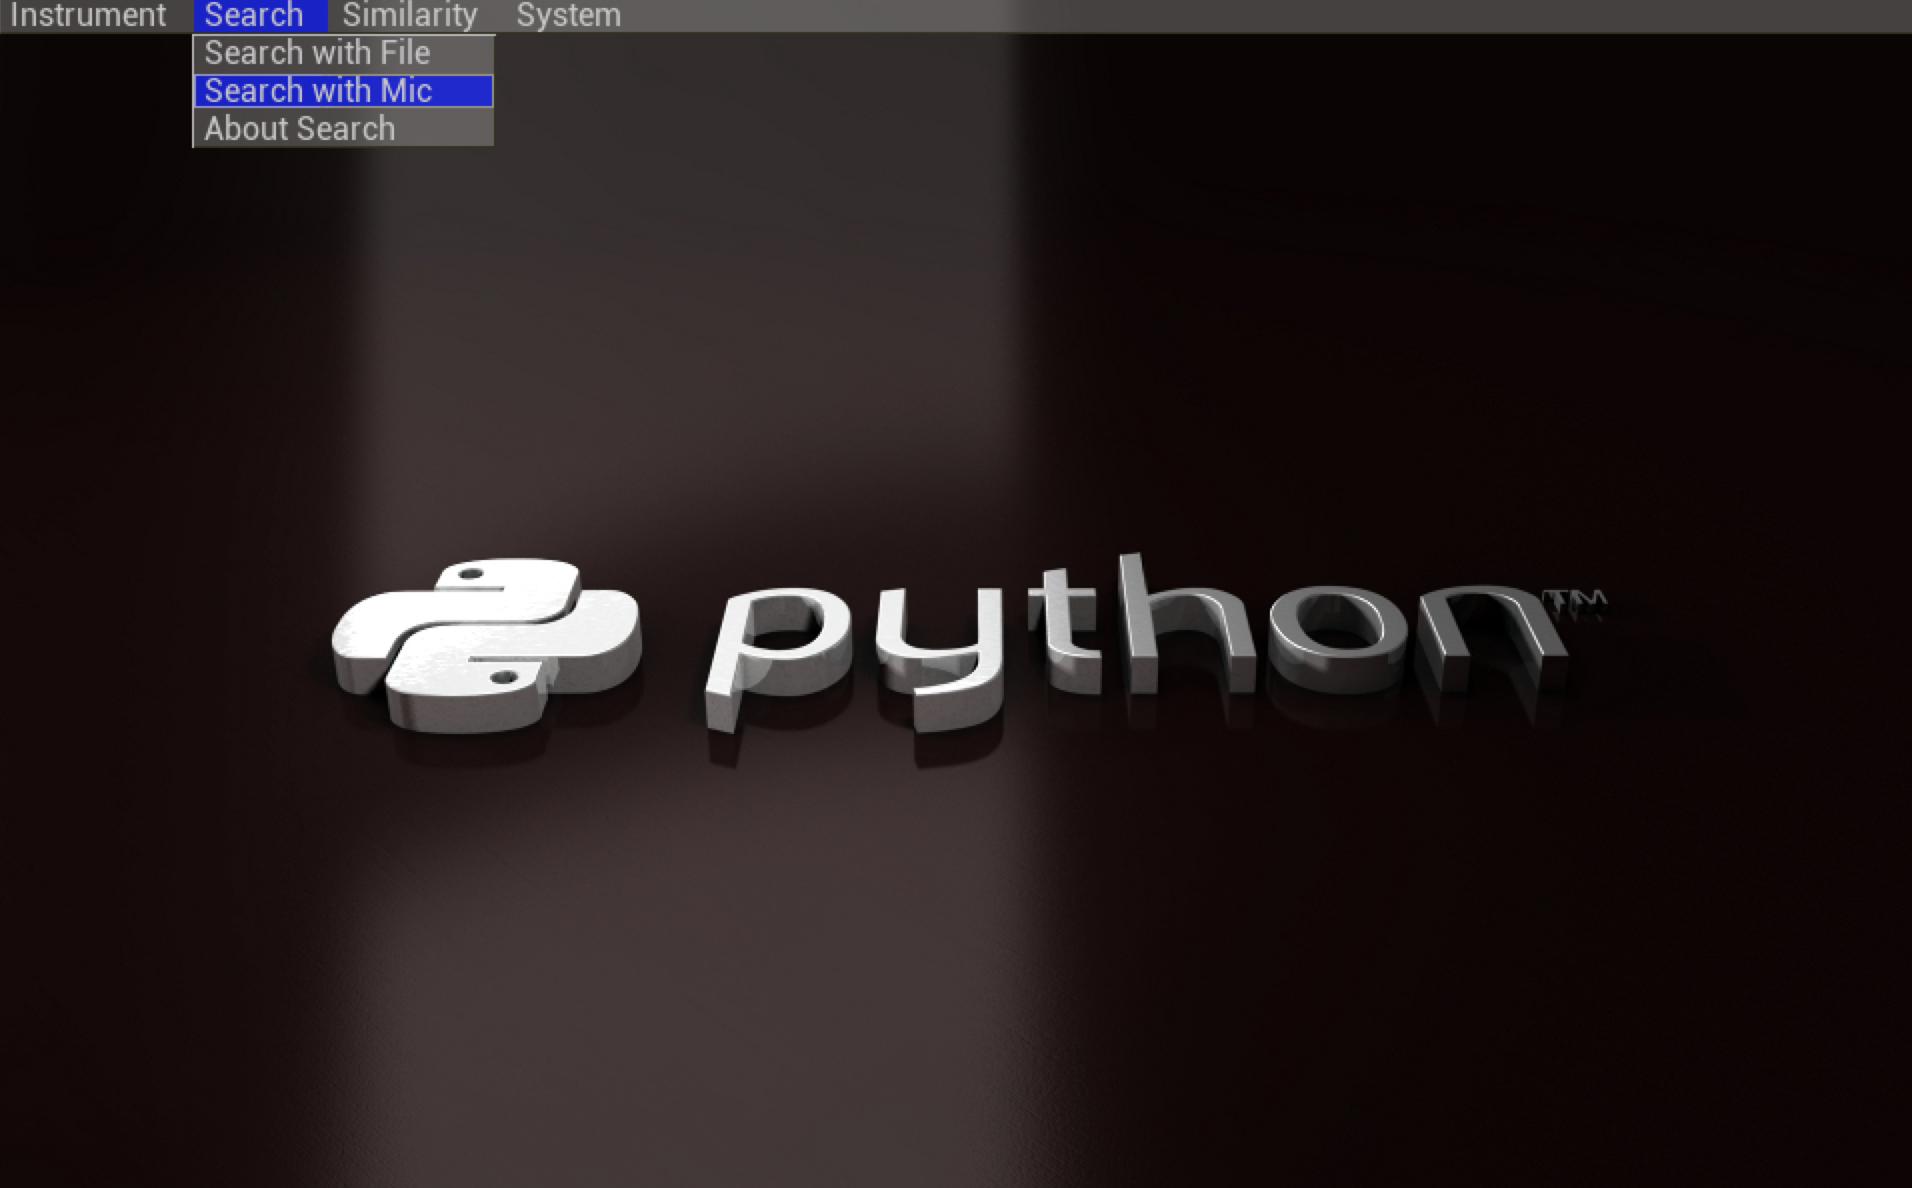
\includegraphics[width=\linewidth]{sm1}
\endminipage\hfill
\minipage{0.497\textwidth}
  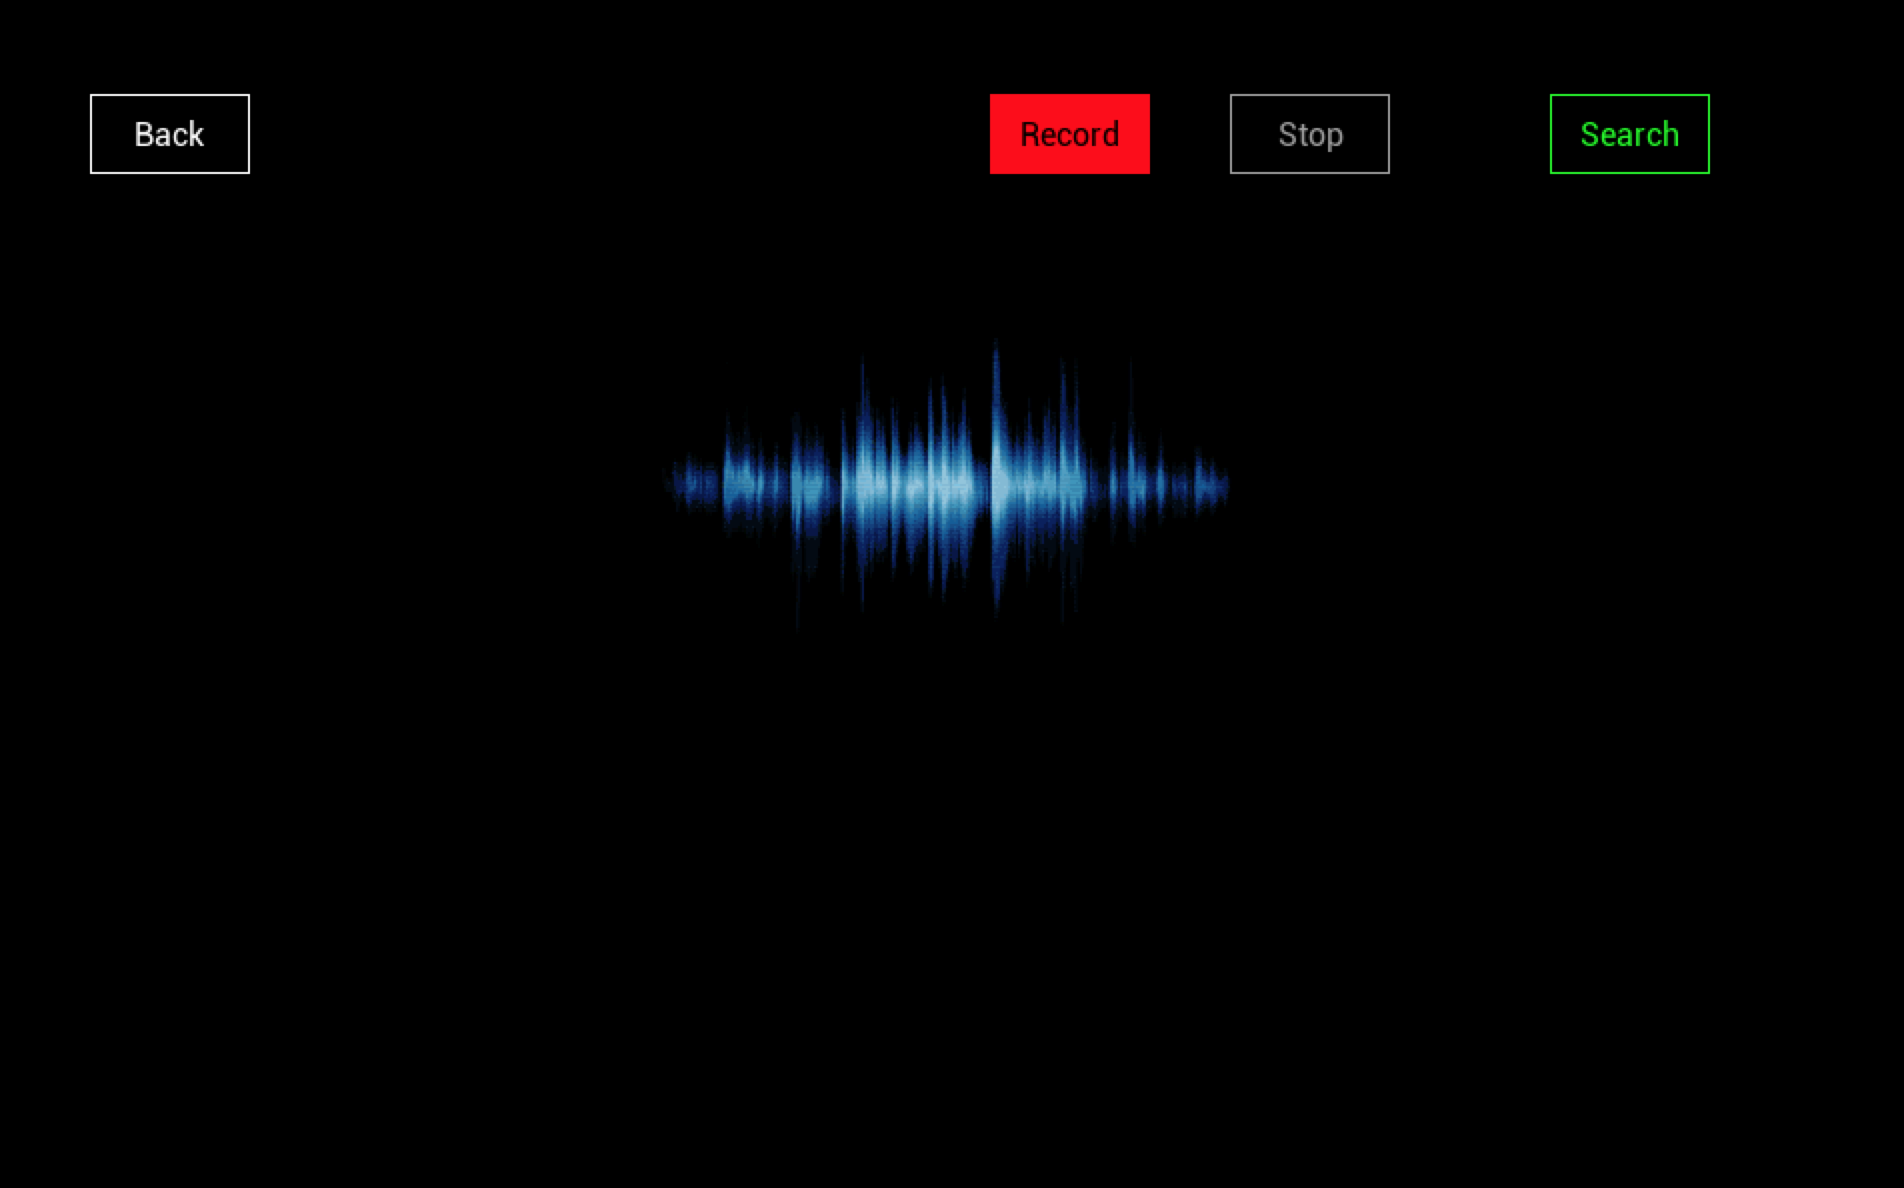
\includegraphics[width=\linewidth]{sm2}
  %\caption{A really Awesome Image}\label{fig:awesome_image2}
\endminipage\hfill\\

\minipage{0.497\textwidth}
  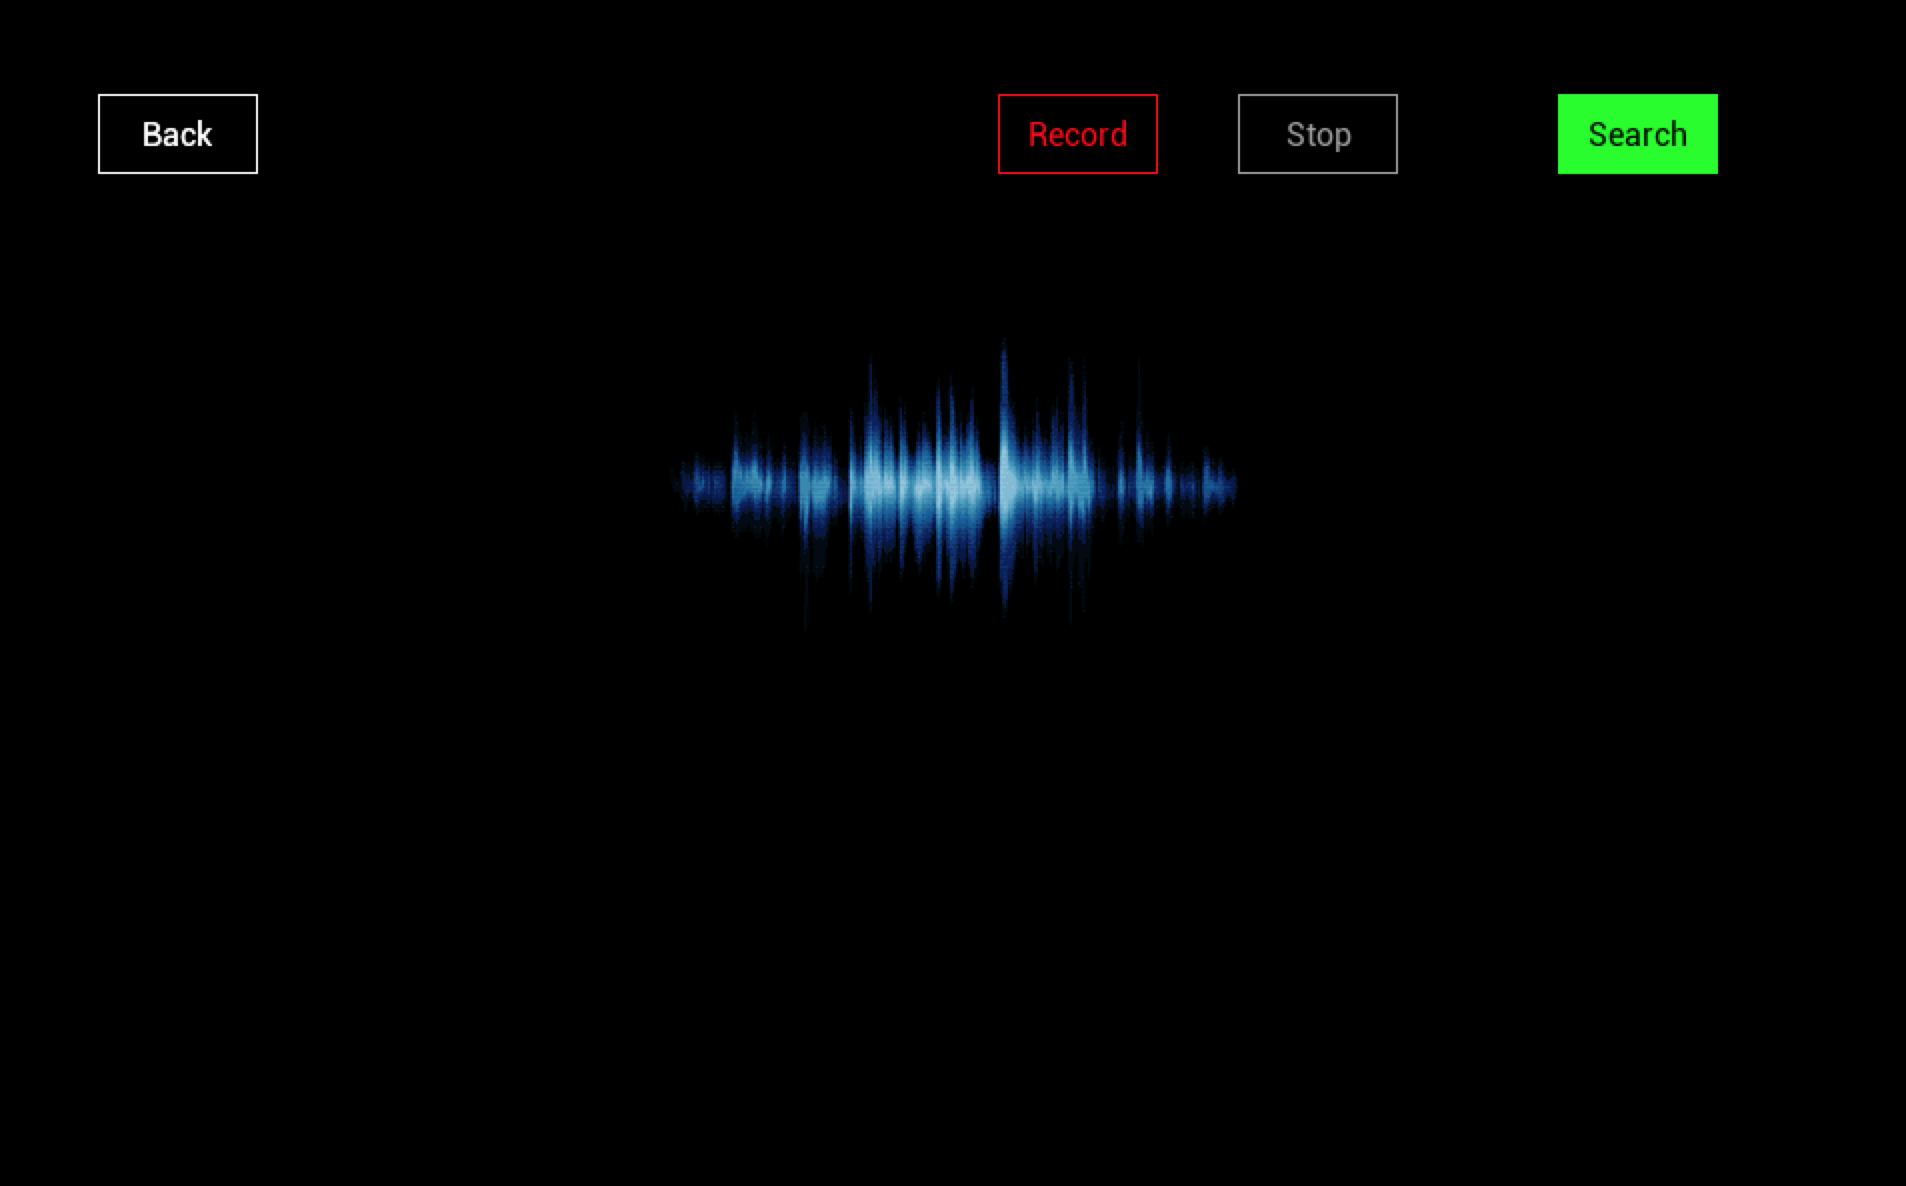
\includegraphics[width=\linewidth]{sm3}
  %\caption{A really Awesome Image}\label{fig:awesome_image2}
\endminipage\hfill
\minipage{0.497\textwidth}
  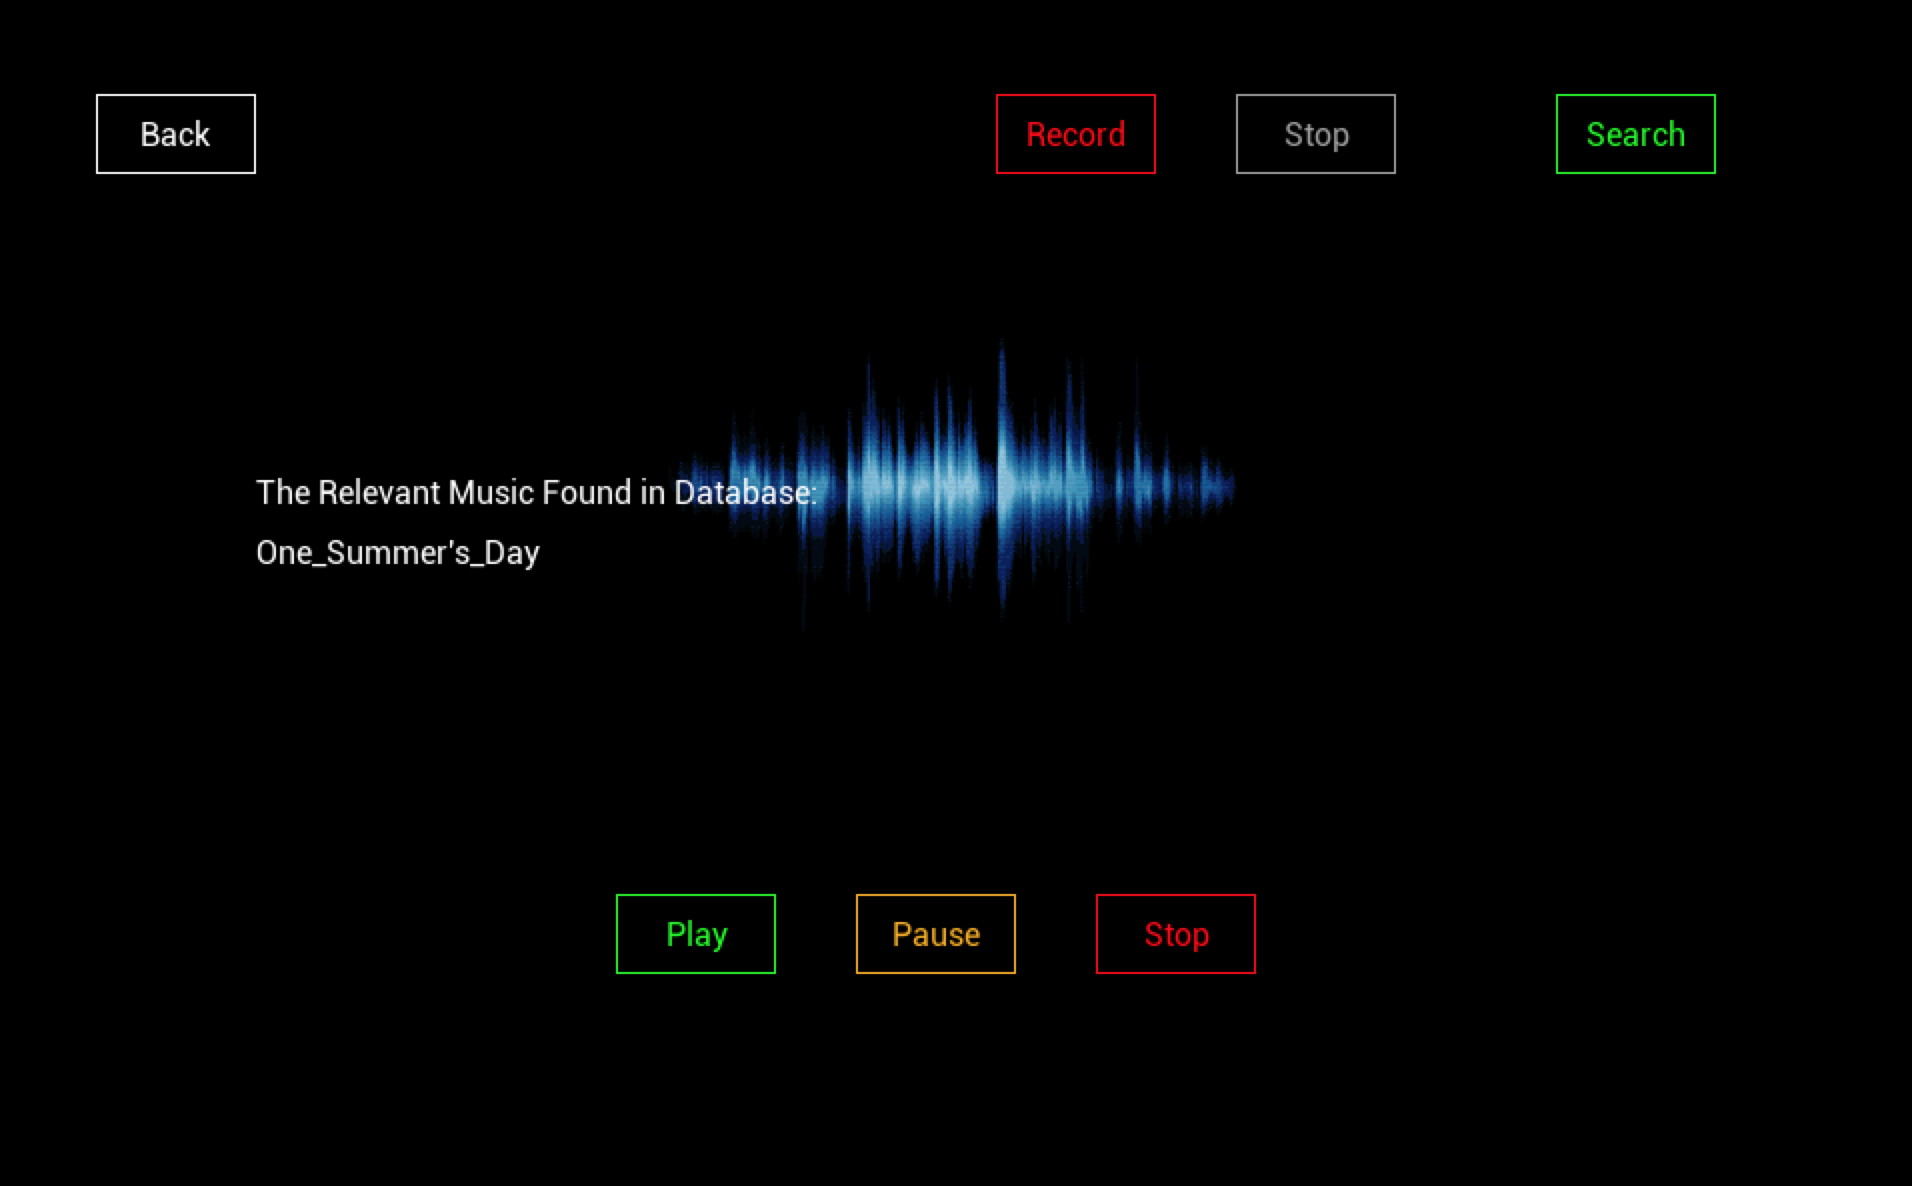
\includegraphics[width=\linewidth]{sm4}
  %\caption{A really Awesome Image}\label{fig:awesome_image2}
\endminipage\hfill

\caption{Walk through of Searching function through microphone. User selects "Search by Mic" in menu, records a clip of  audio, then click on the "Search" button to reveal matching audio.}
\label{fig:sm}
\end{figure}

\section{Rating Plays}
\subsection{Storyboard Walk Through}
\[Insert\_Shots\]

%------------------------------------------------------------------------------------------------------------------------------------
%							Discussion
%------------------------------------------------------------------------------------------------------------------------------------
\chapter{Discussion}
\section{Contribution}
There are three major contributions have been made within this project. 

First of all, not like $c\#$, $python$ is a shell language which contains very few GUI abilities. In a short amount of time, an executable and working $Python$ GUI has been built for integrating with functionality described in Section~\ref{project}. 

Secondly, referring to Ganchev et al. \cite{ganchev2005}, a different tweak on implementing MFCCs is written from scratch, which suits the purpose of classifying instruments in classical music. Besides, a recreation of combining MFCC with Random Forest on instrument recognition, which mentioned in \cite{li2015}, has been successfully produced.

Last but not least, there are very few music applications are focusing on  classical music. Under this circumstance, this project provides an integration of audio processing  on this kind of area.

\section{Reflection and Future Work}
While we were developing objectives of this project, we have gained more insight on how audios are being processed and extracted. In both theoretical and practical concepts, searching functions and instrument recognition have been approved in many sources. However, this is an application that lacks of resource supports. That is, the quantity of songs in our database is inadequate (around 40 songs) since we are collecting and labeling audio data by ourselves. As a consequence, matching results have a possibility that produces a large number of false positives in terms of both searching and classifying aspects. \\
\\
For future implications, it is crucial to expand the size of existing audio resources for minimizing false positives produced by system. Besides, the next step of our application is to identify multiple instruments contained in  mixed audios, since current version is detecting single instrument in audio clips.  In addition, this application is only focusing on classical music since the workloads for covering multiple kinds of music are exceeding the effort we could make within a certain amount of time. Therefore, current system can be extended for exploring different types of music.


%------------------------------------------------------------------------------------------------------------------------------------
%							Conclusion
%------------------------------------------------------------------------------------------------------------------------------------
\chapter{Conclusion}
In this project, an integrated application for identifying and classifying classical music is delivered in following two aspects, $Shazam$-like audio searching and instrument extraction / classification. In terms of instrument extraction, the combination of MFCCs and Random Forest classification has shown a reasonable approach based on empirical experiments. On the other hand, rapid development on audio fingerprints demonstrated promising matching results. However, due to the limitation of resources, other classification technique such as convolution neural network (CNN) is given up in this version of system. To sum up, both existing empirical techniques, audio fingerprinting and MFCCs, have shown strong strength on audio matching and recognizing. in addition, improving current system with the concept of CNN can be carried out once expanding enough size of training data sets.




%% Use letters for the chapter numbers of the appendices.
\appendix
%\input{appendix-a}

\bibliography{report}

\end{document}

